\documentclass[11pt,reqno]{amsart}
\usepackage[T1]{fontenc}
\usepackage{lmodern,amsmath,amssymb,amsthm,mathtools,microtype}
\usepackage[a4paper,margin=29mm]{geometry}
\usepackage{tikz}
\usetikzlibrary{arrows.meta,positioning,calc,fit,backgrounds,patterns}
\usepackage{xcolor,booktabs,enumitem}
\usepackage[colorlinks=true,linkcolor=blue!55!black,citecolor=blue!55!black,urlcolor=blue!55!black]{hyperref}
\usepackage[nameinlink,noabbrev]{cleveref}
\numberwithin{equation}{section}
\newtheorem{theorem}{Theorem}[section]
\newtheorem{proposition}[theorem]{Proposition}
\newtheorem{lemma}[theorem]{Lemma}
\newtheorem{corollary}[theorem]{Corollary}
\theoremstyle{definition}
\newtheorem{definition}[theorem]{Definition}
\newtheorem{example}[theorem]{Example}
\theoremstyle{remark}
\newtheorem{remark}[theorem]{Remark}
\newcommand{\Z}{\mathbb Z}
\newcommand{\N}{\mathbb N}
\newcommand{\E}{\mathbb E}
\newcommand{\Prob}{\mathbb P}
\newcommand{\one}{\mathbf1}
\newcommand{\Gibbs}{\mathcal G}
\newcommand{\cP}{\mathcal P}
\newcommand{\cT}{\mathcal T}
\newcommand{\Cov}{\operatorname{Cov}}
\newcommand{\osc}{\operatorname{osc}}
\newcommand{\diam}{\operatorname{diam}}
\newcommand{\dist}{\operatorname{dist}}
\newcommand{\supp}{\operatorname{supp}}
\newcommand{\TV}{\operatorname{TV}}
\newcommand{\HALT}{\mathsf{HALT}}
\newcommand{\REJECT}{\mathsf{REJECT}}
\newcommand{\vac}{\mathord\varnothing}
\newcommand{\norm}[1]{\lVert#1\rVert}
\newcommand{\abs}[1]{\lvert#1\rvert}
\setlist[enumerate]{label=\textup{(\roman*)},leftmargin=*,itemsep=3pt}
\setlist[itemize]{leftmargin=*,itemsep=3pt}
\hypersetup{pdftitle={Finite Certificates and Undecidable Gibbs Uniqueness},pdfauthor={Harjas Sandhu}}
\title[Finite certificates and Gibbs uniqueness]{Finite Certificates and Undecidable Gibbs Uniqueness}
\author{Harjas Sandhu}
\address{The University of Queensland}
\email{harjas.sandhu@student.uq.edu.au}
\date{6 November 2026}
\subjclass[2020]{Primary 82B20, 03D35; Secondary 60K35, 68Q17, 82B26}
\keywords{Gibbs uniqueness, undecidability, finite-energy lattice models, disagreement percolation, computable equilibrium, pressure}
\begin{document}
\raggedbottom
\begin{abstract}
We construct translation-invariant classical interactions on $\Z^2$ for which deciding uniqueness among all Gibbs states is undecidable at inverse temperature one. The finite on-site alphabet depends effectively on the input; interaction supports are fixed, and local energy terms take only the integer values $0,1,20$. Exact character orthogonality converts a strictly positive finite-energy model into a gas of finite computation histories. A halting certificate produces a uniformly positive phase-selection bias, however small. A reference Ising comparison and an independent-disagreement argument then give uniqueness and exponential clustering of every local physical observable. Without halting, the entire Gibbs simplex is affinely isomorphic to the two-dimensional zero-field Ising simplex. A distinct soft-certificate construction has the same dichotomy for one table at every finite inverse temperature at least $2/5$. We prove boundary-specific exponential convergence, smooth pressure with summable cumulants on the uniqueness branch, uniform computability of the selected phase and its right pressure jet, and stability under small finite-range spin perturbations. An effective compactness argument supplies a computable valid convergence modulus for each unique computable finite-range specification; the impossibility concerns total bounds across the undecidable family. Exact microscopic symmetrization excludes a family-wide perturbation radius for arbitrary real interactions.
\end{abstract}
\maketitle
\setcounter{tocdepth}{1}
\tableofcontents
\clearpage

% Section: overview
\section*{Conceptual overview}
\label{sec:overview}

The main construction turns one question about a computation into one question about equilibrium: does the entire physical Gibbs simplex contain one state or more than one? The compiler outputs a finite interaction without deciding which outcome occurs. At inverse temperature $\beta=1$, its physical weights are strictly positive, its local energy terms lie in $\{0,1,20\}$, and only the finite on-site alphabet depends on the machine and input.

\begin{center}
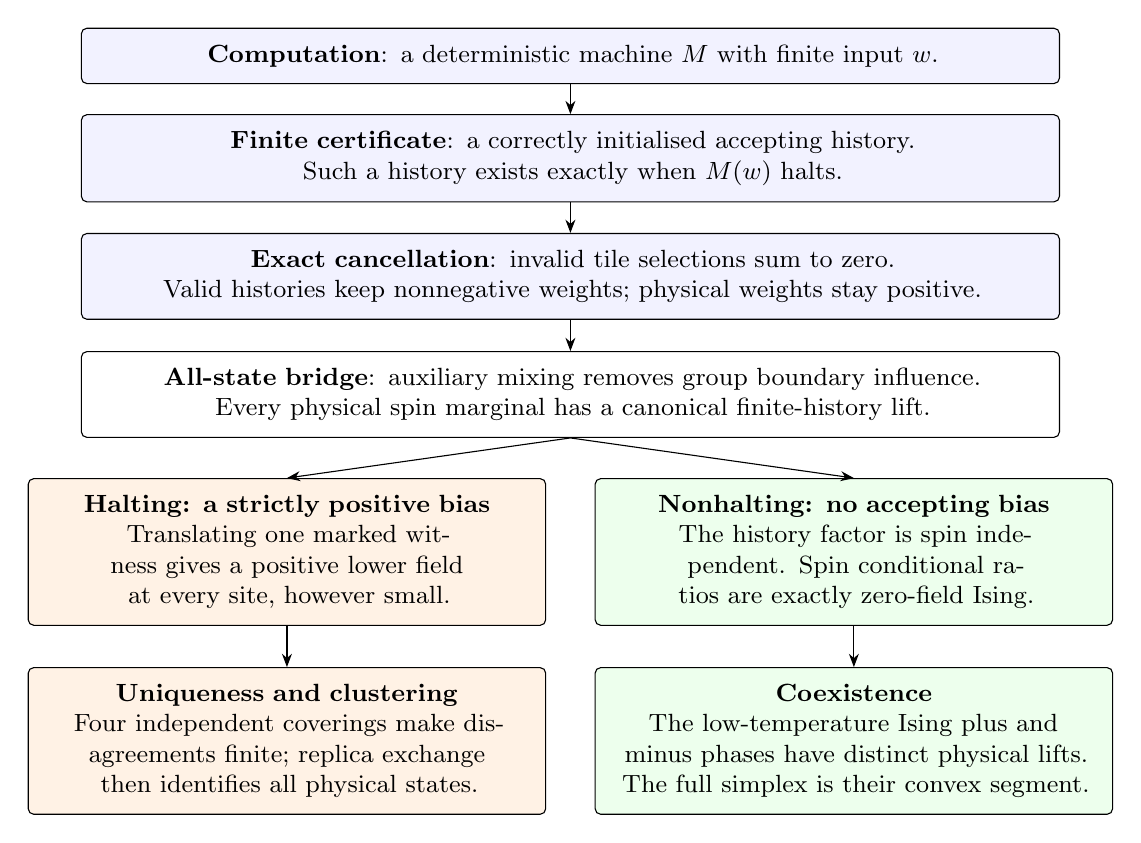
\begin{tikzpicture}[
 font=\small,>=Stealth,
 stage/.style={draw,rounded corners=2pt,align=center,inner sep=6pt,text width=12.0cm},
 branch/.style={draw,rounded corners=2pt,align=center,inner sep=6pt,text width=6.15cm}]
 \node[stage,fill=blue!5] (machine) at (0,0)
 {\textbf{Computation}: a deterministic machine $M$ with finite input $w$.};
 \node[stage,fill=blue!5] (certificate) at (0,-1.3)
 {\textbf{Finite certificate}: a correctly initialised accepting history.\\
 Such a history exists exactly when $M(w)$ halts.};
 \node[stage,fill=blue!5] (cancel) at (0,-2.8)
 {\textbf{Exact cancellation}: invalid tile selections sum to zero.\\
 Valid histories keep nonnegative weights; physical weights stay positive.};
 \node[stage] (bridge) at (0,-4.3)
 {\textbf{All-state bridge}: auxiliary mixing removes group boundary influence.\\
 Every physical spin marginal has a canonical finite-history lift.};
 \node[branch,fill=orange!10] (bias) at (-3.6,-6.3)
 {\textbf{Halting: a strictly positive bias}\\
 Translating one marked witness gives a positive lower field at every site, however small.};
 \node[branch,fill=green!7] (zero) at (3.6,-6.3)
 {\textbf{Nonhalting: no accepting bias}\\
 The history factor is spin independent. Spin conditional ratios are exactly zero-field Ising.};
 \node[branch,fill=orange!10] (unique) at (-3.6,-8.7)
 {\textbf{Uniqueness and clustering}\\
 Four independent coverings make disagreements finite; replica exchange then identifies all physical states.};
 \node[branch,fill=green!7] (coexist) at (3.6,-8.7)
 {\textbf{Coexistence}\\
 The low-temperature Ising plus and minus phases have distinct physical lifts. The full simplex is their convex segment.};
 \draw[->] (machine)--(certificate);
 \draw[->] (certificate)--(cancel);
 \draw[->] (cancel)--(bridge);
 \draw[->] (bridge.south)--(bias.north);
 \draw[->] (bridge.south)--(zero.north);
 \draw[->] (bias)--(unique);
 \draw[->] (zero)--(coexist);
\end{tikzpicture}
\end{center}

\noindent\textbf{Where exactness matters.}
An arbitrarily small uncompensated accepting weight would already produce a false positive field on a nonhalting input. \Cref{ex:false-certificate} computes this error explicitly. Cancellation concerns signed terms in an expansion of positive weights; it does not forbid any physical configuration.

\smallskip
\noindent\textbf{Construction, refinements and established inputs.}
The exact-table reduction is the principal construction (\cref{thm:hard}). A separate soft table and its common temperature interval refine it (\cref{thm:soft}); convergence, pressure and perturbation results come afterwards (\cref{thm:consequences}). Ising uniqueness and classification, Dobrushin comparison and finite replica exchange are established machinery. The contribution is their verified connection to the finite-temperature computational encoding and to \emph{all} physical Gibbs states.

\clearpage

% Section: introduction
\section{Introduction and principal results}\label{sec:intro}

Uniqueness of a Gibbs state asks whether every boundary condition leads to the same infinite-volume equilibrium. It is a statement about an entire specification, not merely about decay of correlations in one chosen phase. At low temperature the two-dimensional Ising model illustrates the distinction: its plus phase clusters, yet a different minus phase exists. We show that this distinction can encode an arbitrary halting problem even when the microscopic data are exact integers and the temperature is fixed in advance.

The principal construction is \cref{thm:hard}. Its contribution is the conjunction of fixed positive temperature, strictly positive physical weights, a fixed finite integer-energy palette, and a halting reduction for uniqueness among \emph{all} DLR states. Computation in lattice rules and the probabilistic tools used below have earlier precedents; the finite-table encoding and its all-state physical projection are the interfaces proved here. The \hyperref[sec:overview]{conceptual overview} displays the complete argument before its technical development.

The computational information enters through finite certificates: correctly initialised finite histories containing a halting event. Directly rewarding a local approximation to such a history is inadequate at positive temperature, where every finite pattern, including an erroneous one, has positive probability. Instead we arrange an exact algebraic cancellation. Auxiliary finite-group characters cancel every finite tile selection with an unmatched boundary or inconsistent local colours. The surviving terms are nonnegative weights of valid finite computation histories. The microscopic model nevertheless has no forbidden configurations and no infinite energy.

A certificate may be extremely large, and its induced bias arbitrarily small. A uniform high-temperature estimate for the distinguished spins is consequently unavailable. We use the bias only to select the plus phase of a low-temperature Ising reference. The reference supplies rare contours. Independently, computation histories are covered by a dilute family of finite objects. Two replicas yield four independent covering families. Their subcritical overlap graph makes every disagreement component finite, permitting a finite replica exchange and proving uniqueness for arbitrary Gibbs states. The exchange principle is established machinery; the independent covering construction and its connection to the positive physical model are additional steps. \Cref{ex:false-certificate} isolates the need for an exact zero, and \cref{sec:geometricidea} explains the geometry of the coverings and replica exchange before the estimates.

\subsection{Conventions}
An interaction on a finite alphabet $\mathcal A$ assigns finite real functions $\Phi_X$ to finite $X\subset\Z^2$. Our interactions are translation invariant and have fixed finite range. For finite $\Lambda$, $H_\Lambda^\tau$ is the sum of terms meeting $\Lambda$, with exterior configuration $\tau$. The Gibbs kernel is proportional to $\exp(-\beta H_\Lambda^\tau)$; a Gibbs state satisfies all these local conditional identities (the DLR equations). No invariance is imposed on a Gibbs state. A dimensionless field multiplies the weight by $\exp(\sum_x H_xs_x)$.

Distances and diameters use the $\ell^\infty$ metric, unless described as nearest-neighbour adjacency. For finite $A$, $A^+$ is its closed nearest-neighbour collar: $|A^+|\leq5|A|$ and $\diam A^+\leq\diam A+2$. Put $K=20\beta$. An Ising bond contributes $\exp(-K\one_{s_x\ne s_y})$; the conventional exponent coupling is $J=K/2$.

Effectiveness means that a finite table is computable from the input, not that its construction is efficient. Computability assertions require computable parameters, or effective names for them. Qualitative assertions hold for arbitrary real parameters in the stated ranges. Computability of a state means computability of its cylinder probabilities, equivalently of expectations of local observables with computable finite tables; covariance bounds allow arbitrary bounded local observables.

\subsection{Main theorem: the integer-energy construction}
The first theorem contains the undecidability construction. Its input is a finite machine description, and its output is an exact finite physical interaction; no coupling is specified by an oracle for a halting time.

\begin{theorem}[Fixed-temperature undecidability]\label{thm:hard}
An algorithm takes a deterministic Turing machine and its finite input to a finite alphabet with a distinguished coordinate $s_x\in\{-1,1\}$ and a translation-invariant interaction on $\Z^2$ with support shapes
\[
 \{0,-e_1,-e_2\},\qquad \{0,e_1\},\qquad \{0,e_2\}.
\]
The displayed local terms have energy values in $\{0,1,20\}$. At $\beta=1$:
\begin{enumerate}
\item Without halting, spin projection is an affine bijection from the entire physical Gibbs simplex onto the zero-field nearest-neighbour Ising Gibbs simplex with mismatch exponent $20$.
\item With halting, there is exactly one physical Gibbs state. Every pair of bounded local physical observables has exponentially decaying connected correlation.
\end{enumerate}
Thus full Gibbs uniqueness is undecidable for these exact finite tables. Without halting there are exactly two extremal Gibbs states; their equal mixture has spin covariance bounded away from zero at arbitrary separation.
\end{theorem}

\subsection{A refinement: soft certificates and a temperature interval}
Each accepting history in \cref{thm:hard} imposes a hard plus pin at a single anchor. This constraint belongs to a proof representation, not to the physical model. The next result refines the construction by using a \emph{different} table: a finite penalty replaces each proof pin, unmarked histories are permitted, and one history may contain several marks. Uniform estimates then give a common temperature interval for that table. This is a further construction sharing the same mechanism, not a change to the table in \cref{thm:hard}.

\begin{theorem}[Soft certificates and a common temperature interval]\label{thm:soft}
An effective construction with the same support shapes and energy values has the following properties for the \emph{same table} at every finite $\beta\geq2/5$.
\begin{enumerate}
\item Without halting, its entire physical Gibbs simplex is the affine lift of the zero-field Ising simplex with mismatch exponent $K=20\beta$.
\item With halting, its entire physical Gibbs simplex is a singleton, exponentially clustering for all bounded local physical observables. For spin observables on $A,B$,
\begin{equation}\label{eq:maincov}
 |\Cov(f,g)|\leq4\norm f_\infty\norm g_\infty |A||B|2^{-\dist(A,B)}.
\end{equation}
\item At each fixed $\beta$, a witnessed marked history determines $h_*=h_*(\beta,\gamma_*)>0$ such that uniqueness and the same spin bound hold for every bounded inhomogeneous field with $\inf_x H_x>-h_*$. For uniform $h>-h_*$, the physical pressure is $C^\infty$, with absolutely convergent cumulant formulas and $0\leq p_\beta''(h)\leq68$.
\end{enumerate}
The physical clustering exponent is uniformly positive, independently of the halting time. The field margin $h_*$ need not be bounded below across inputs.
\end{theorem}

At zero field, for both constructions the nonhalting simplex is a segment and the halting simplex a point. Every Gibbs state is translation invariant. Each nonhalting endpoint clusters; an interior mixture does not. The existence of a clustered phase alone therefore does not distinguish the cases.

The Ising segment classification in this statement is an application of Aizenman--Higuchi. What must be supplied for the physical model is the inverse affine projection and lift, including arbitrary, potentially non-translation-invariant Gibbs states; this is proved in \cref{sec:allprojection}.

\subsection{Further results and corollaries}
The following results describe what can be deduced or further proved once the construction is available. They do not constitute additional encodings of computation. In particular, computable pressure and smooth-response techniques have established predecessors; the new obligations here are their precise applicability and effectiveness for this family. The perturbation result requires an additional activation argument and retains its spin-only scope.

\begin{theorem}[Effectiveness, pressure and stability]\label{thm:consequences}
For the models and temperatures in \cref{thm:hard,thm:soft}:
\begin{enumerate}
\item Plus-spin boxes with freely summed incident group variables converge exponentially to a selected physical Gibbs state, uniformly over machine inputs. This state is uniformly computable. On a halting input, convergence is also exponential for arbitrary spin boundaries with these free group variables, with model-dependent constants.
\item The pressure is uniformly computable. All right derivatives at zero exist and form a uniformly computable smooth right jet. Zero-field differentiability is equivalent to halting. The left derivative is not uniformly computable across the family.
\item On a halting input, sufficiently small finite-range spin-only multibody perturbations preserve uniqueness and exponential clustering. An explicit sufficient radius depends on a witnessed history and the perturbation range. At $\beta=1$ there is no positive family-wide radius for arbitrary real perturbations of the physical interaction.
\end{enumerate}
Every unique computable finite-alphabet, finite-range, finite-energy specification has a computable valid all-boundary convergence modulus, found by one partial algorithm under the uniqueness promise. No total algorithm on the whole machine family can supply a valid minus-boundary or all-boundary bound on every halting input.
\end{theorem}

The boundary qualifications are part of these conclusions. We prove neither strong spatial mixing for arbitrary microscopic boundaries nor a Glauber mixing-time bound. Smooth pressure does not here imply analyticity.

\subsection{Relation to earlier work}
Computation in local lattice rules begins with the domino problem \cite{Berger1966}. Wolfram \cite{Wolfram1985} discussed undecidability and intractability in physical lattice models; Kanter \cite{Kanter1990} treated computational unpredictability in classical systems. Ground-state encodings by Gu et al.\ \cite{GuWeedbrookPeralesNielsen2009} and Gu--Perales \cite{GuPerales2012}, and the characterization of multidimensional shift entropies by Hochman--Meyerovitch \cite{HochmanMeyerovitch2010}, show the strength of computational encodings at zero temperature or with forbidden patterns. Quantum spectral-gap undecidability \cite{CubittPerezGarciaWolf2022} concerns a distinct problem. None of these statements is used here as a finite-temperature uniqueness theorem. We make no general priority claim over all formulations of undecidability in statistical mechanics.

The finite-temperature construction combines a positive exact integer table, character cancellation, an all-state projection and lift, and phase selection by a finite certificate of unbounded possible size. The full Ising classification is an application of Aizenman--Higuchi in the form of Coquille--Velenik \cite[Corollary~1.1]{CoquilleVelenik2012}. Positive-field reference uniqueness uses Lebowitz--Martin-L\"of \cite[Theorem~1 and p.~278]{LebowitzMartinLof1972} and Lee--Yang \cite{LeeYang1952}. These results are applied to the ferromagnetic reference, never to the projected target.

The replica exchange is van den Berg's independent-disagreement method \cite[Theorem~1]{VanDenBerg1993}. Disagreement percolation \cite{VanDenBergMaes1994} and Dobrushin comparison \cite{Dobrushin1968,RebeschiniVanHandel2014} supply its context. We give the exchange and its independent covering construction explicitly. A finite-gas exchange also constructs the canonical history gas without a cluster expansion. Koteck\'y--Preiss \cite{KoteckyPreiss1986} and Ferrari--Fern\'andez--Garcia loss networks \cite{FerrariFernandezGarcia2002} are applicable alternatives, not new principles.

Clustering-to-smoothness arguments are classical \cite{Lebowitz1972Correlations,LebowitzPenrose1968}. We establish the inhomogeneous uniformity and finite-tilt limit required in this model. Computability of pressure and equilibrium states has a substantial existing theory \cite{GayralSablikTaati2025,BinderHeLiZhang2025,FawziFawziScalet2024}. Our compactness certificate concerns all DLR boundaries and identifies the convergence obstruction compatible with uniqueness. Exact applicability statements appear in \cref{app:imports}.

Three representations remain distinct throughout. The physical alphabet has positive weights. Conditional on spins its group variables are uniformly mixing. Free group summation then represents spin ratios by a separate positive history gas. Only its canonical finite-component sector is used. Infinite formal tilings are not identified with extra physical Gibbs states.


% Section: construction
\section{Finite histories and positive integer energies}\label{sec:construction}

\subsection{Two finite-certificate grammars}
A deterministic machine can be made total with absorbing states $\HALT$ and $\REJECT$. Fold its two-sided tape onto the nonnegative integers, storing the original cells $j$ and $-j-1$ together. A permanent origin bit permits a radius-one rule to distinguish a track change at the origin from a move elsewhere. A proposed move through a wall becomes $\REJECT$, even if the proposed transition would halt. This prevents finite-width artefacts from becoming certificates. The full finite grammar appears in \cref{app:compiler}.

Both grammars have finite labelled Wang-tile sets $\cT$ with a zero boundary colour. A finite nonzero-edge component with zero exterior must be a solid rectangle of width and height at least two. Its bottom row is the entire prescribed input followed by blanks, and subsequent rows are its exact deterministic bounded-width evolution. A finite automaton accepting precisely $Pz^*$ implements the bottom condition, where $P$ is the prescribed initial word and $z$ an ordinary blank cell.

In the \emph{hard, single-anchor grammar}, the top row must contain exactly one halting head and no other head. The top-left tile is marked. Every finite component has one mark, and a finite component exists exactly when the computation halts. In the \emph{soft grammar}, the top automaton accepts every word; a tile is marked precisely when its centre cell carries a halting head. Unmarked prefixes and rejecting histories are allowed. A marked component exists exactly when the computation halts. Absorption of the halting state permits several marks in one component.

Colours force the full rectangle and computation, not merely plausible transitions. Nonzero matching cannot terminate at a hole or produce a ragged boundary. Components may touch across zero-coloured edges without merging.

\begin{figure}[ht]
\centering
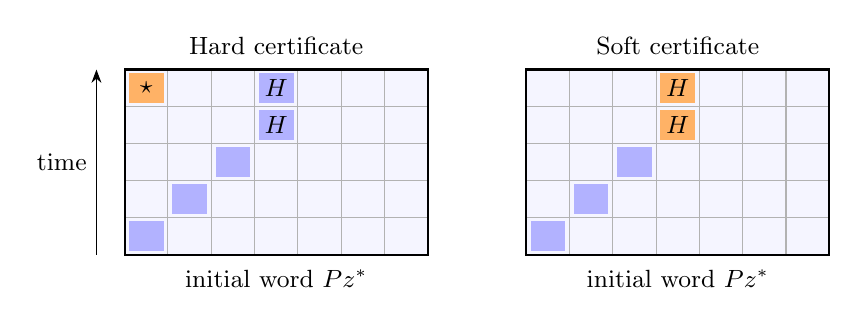
\begin{tikzpicture}[x=.55cm,y=.47cm,font=\small]
 \foreach \shift/\kind in {0/Hard,5.1/Soft} {
  \begin{scope}[xshift=\shift cm]
   \node at (3.5,5.65) {\kind\ certificate};
   \fill[blue!4] (0,0) rectangle (7,5);
   \foreach \x/\y in {0/0,1/1,2/2,3/3,3/4}
    {\fill[blue!30] (\x+.1,\y+.1) rectangle (\x+.9,\y+.9);}
   \ifdim\shift pt=0pt
    \fill[orange!60] (.1,4.1) rectangle (.9,4.9);
    \node at (.5,4.5) {$\star$};
   \else
    \foreach \y in {3,4}
     {\fill[orange!60] (3.1,\y+.1) rectangle (3.9,\y+.9);}
   \fi
   \foreach \y in {3,4} {\node at (3.5,\y+.5) {$H$};}
   \draw[step=1,gray!60] (0,0) grid (7,5);
   \draw[thick] (0,0) rectangle (7,5);
   \node at (3.5,-.65) {initial word $Pz^*$};
  \end{scope}
 }
 \draw[-{Stealth}] (-.65,0)--node[left]{time}(-.65,5);
\end{tikzpicture}
\caption{Two certificate tables for the same schematic history. Blue cells trace the head, and $H$ denotes an absorbing halting head. Orange marks are the single top-left anchor in the hard table and all halting centres in the soft table. The exact finite rule is given in \cref{app:compiler}.}
\label{fig:histories}
\end{figure}

\par\noindent
\begin{minipage}{\textwidth}
\subsection{Why a rare false certificate is still an error}
\begin{example}[A false accepting mark and its exact cancellation]\label{ex:false-certificate}
Consider a toy marker at one spin, with relative weight $w>0$ when the spin is plus and $rw$ when it is minus, where $0<r<1$. The empty marker has weight one. Summing the marker gives
\[
 Z_+=1+w,\qquad Z_-=1+rw,\qquad
 h_{\rm err}=\frac12\log\frac{1+w}{1+rw}>0.
\]
With $w=1/100$ and $r=1/2$, for instance, the false field is exactly $\frac12\log(202/201)$. If the marker represents an invalid computation that has merely been assigned a finite penalty $E$, then $w=e^{-\beta E}$ remains positive at every finite $E$. Putting this same independent marker at every site of low-temperature zero-field Ising produces a positive uniform field after summation, and therefore selects a unique reference equilibrium. Its rarity has not preserved the intended nonhalting coexistence branch. This calculation concerns an uncompensated accepting weight; it does not rule out other encodings that correct or balance errors.

Here is the local operation that instead gives zero. Suppose neighbouring pieces of a proposed history assign different bits, $1$ and $0$, to their common edge. On $G=\Z/2\Z$, set $\chi_0(g)=1$ and $\chi_1(g)=(-1)^g$. The shared-edge average distinguishes the invalid pair from a matching pair:
\[
 \begin{array}{c|cc|c}
  \text{selected colours}&g=0&g=1&\text{average}\\ \hline
  (1,0)&1&-1&0\\
  (1,1)&1& 1&1
 \end{array}
\]
Thus the contradictory local claim has zero contribution, rather than a small positive one. There is no negative physical probability: for $0<\varepsilon<1$, both factors $1+\varepsilon\chi_c(g)$ and $1+\varepsilon\chi_d(g)$ are positive, while their selected cross-term $\varepsilon^2\chi_c(g)\chi_d(g)$ has zero average when $c\ne d$.

In the full construction the grammar checks initialisation, transitions and acceptance. Shared-edge cancellation enforces the required colour equalities, and dangling-edge cancellation enforces the exterior boundary. Every surviving marked object is therefore a genuine certificate. Valid unmarked histories in the soft version may survive; an invalid accepting history may not. All physical configurations still have positive weight.
\end{example}
\end{minipage}
\par\medskip

\subsection{The positive physical table}
Let $t=|\cT|$. Assign each colour $c$ a distinct real character $\chi_c$ of $G=(\Z/2\Z)^m$, with zero assigned the trivial character. Choose $2^m$ at least the number of colours. One $G$ variable lies on each nearest-neighbour edge, shared by its endpoints. For a tile $z$ at $v$, put
\[
 \mathcal X_{v,z}(g)=\prod_{e\ni v}\chi_{c(z,e)}(g_e).
\]
Use $(p,q)=(1,0)$ for the hard grammar and $(p,q)=(2,1)$ for the soft grammar. Set $r=q/p$ and
\[
 c_z(s)=\begin{cases}q,&z\text{ marked and }s=-1,\\p,&\text{otherwise},\end{cases}
 \quad F_v(g,s)=\sum_{z\in\cT}c_z(s_v)\mathcal X_{v,z}(g),\quad L=pt.
\]
Thus $F_v$ is integral and $|F_v|\leq L$. Define
\begin{equation}\label{eq:integer-table}
 C_0=10000(L+1),\quad D=C_0+L,\qquad
 E_v=\one_{\{b_v>C_0+F_v(g,s)\}},\quad b_v\in\{1,\ldots,D\}.
\end{equation}
The Hamiltonian sums these $0$--$1$ terms and $20\one_{s_x\ne s_y}$ over bonds. Store east and north group variables at their left or lower endpoints. The alphabet is
\begin{equation}\label{eq:alphabet}
 \mathcal A=\{-1,1\}\times\{1,\ldots,D\}\times G^2.
\end{equation}
The site factor has support $\{v,v-e_1,v-e_2\}$; the bond terms have the two pair supports. This is a finite algorithmic table requiring no halting-time estimate. Every physical configuration has positive weight at finite temperature.

Summing the multiplicity variable gives exactly
\begin{equation}\label{eq:multiplicity}
 \sum_{b_v=1}^D e^{-\beta E_v}
 =C_\beta(1+a_\beta F_v),\qquad
 C_\beta=C_0+Le^{-\beta},\quad
 a_\beta=\frac{1-e^{-\beta}}{C_\beta},\quad u=La_\beta<10^{-4}.
\end{equation}
The noninteger quantities here are derived weights, not microscopic couplings. Put $\lambda=pa_\beta$, so $t\lambda=u$.

\subsection{Exact cancellation and the positive gas}\label{sec:fourier}
For a finite set of factor centres $V$, integrate with normalized counting measure over every group edge incident to $V$, including dangling edges. Expand $\prod_{v\in V}(1+a_\beta F_v)$. At each centre no tile or one tile is selected. Orthogonality gives
\begin{equation}\label{eq:orthogonality}
 \int_G\chi_c\chi_d=\one_{c=d},\qquad \int_G\chi_c=\one_{c=0}.
\end{equation}
A selection survives exactly when internal colours match and dangling selected edges have colour zero. The grammar decomposes it into site-disjoint finite labelled rectangles $\gamma$. Denote sites by $S_\gamma$ and marks by $M_\gamma\subset S_\gamma$. With $w_\gamma=\lambda^{|S_\gamma|}$, the exact identity is
\begin{equation}\label{eq:gas}
 \Xi_V(s):=\int\prod_{v\in V}(1+a_\beta F_v(g,s))\,dg
 =\sum_{P:\,S_\gamma\subset V}\prod_{\gamma\in P}w_\gamma r^{N_-(M_\gamma,s)}.
\end{equation}
The sum ranges over site-disjoint objects. For $r=0$ use $0^0=1$: an occupied hard anchor requires plus spin. Every surviving term is nonnegative.

Without halting the hard table gives $\Xi_V=1$, since only the empty selection survives. For the soft table all finite histories are unmarked, so $\Xi_V$ is spin independent but generally not one. Both give exactly the bare Ising spin ratios. These partition identities must not be conflated.

\begin{figure}[ht]
\centering
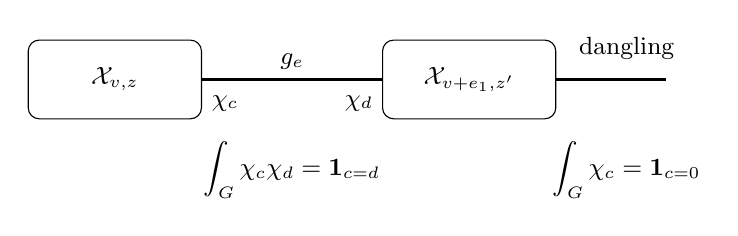
\begin{tikzpicture}[font=\small,>=Stealth]
 \node[draw,rounded corners,minimum width=2.2cm,minimum height=1cm] (l) at (0,0) {$\mathcal X_{v,z}$};
 \node[draw,rounded corners,minimum width=2.2cm,minimum height=1cm] (r) at (4.5,0) {$\mathcal X_{v+e_1,z'}$};
 \draw[thick] (l)--node[above] {$g_e$} (r);
 \node at (1.4,-.3) {$\chi_c$};\node at (3.1,-.3) {$\chi_d$};
 \node at (2.25,-1.15) {$\displaystyle\int_G\chi_c\chi_d=\one_{c=d}$};
 \draw[thick] (r.east)--(7,0);\node at (6.5,.4) {dangling};
 \node at (6.5,-1.15) {$\displaystyle\int_G\chi_c=\one_{c=0}$};
\end{tikzpicture}
\caption{Shared group variables enforce matching, and freely summed dangling variables enforce zero exterior colour. Both are cancellation identities within a positive physical model.}
\label{fig:orthogonality}
\end{figure}

\begin{remark}
Fixed dangling group values and periodic windings do not satisfy \eqref{eq:gas} in this form. We remove arbitrary physical group boundaries by conditional mixing before using free integration. Infinite matching tile planes are allowed by the grammar and are not classified by the finite-component lemma.
\end{remark}


% Section: projection
\section{Canonical objects and projection of every Gibbs state}\label{sec:projection}

\subsection{A canonical gas without a cluster expansion}
Object species are labelled finite supports; incompatibility means overlap. Put $a_\gamma(s)=w_\gamma r^{N_-(M_\gamma,s)}\leq w_\gamma$. Finitely many species lie in a fixed finite spatial volume. The number of size-$n$ species containing a fixed site is at most $(16t)^n$: use a deterministic doubled spanning-tree walk to count the connected support, then label its sites. Thus rooted activity tails are uniformly summable. In particular,
\begin{equation}\label{eq:Bp}
 B_{\rm obj}=2\sup_x\sum_{\gamma:\,x\in S_\gamma}|S_\gamma|w_\gamma2^{\diam S_\gamma}
 \leq2\sum_{n\geq1}n(32u)^n<0.006442.
\end{equation}

\begin{lemma}[Finite-gas exchange]\label{lem:gaslimit}
The free finite gases in \eqref{eq:gas} converge to a measurable canonical law $Q_s$, uniformly over complete spin profiles. Its decoded local patterns depend exponentially weakly on remote volume cutoffs and remote spin changes. It obeys all finite-species insertion and removal identities, and almost surely consists of finite objects. For each $s$ it has a measurable coupling below an independent Bernoulli family $(R_\gamma)$ with parameters $w_\gamma$, whose joint law is independent of $s$.
\end{lemma}
\begin{proof}
Given all other species, occupation of $\gamma$ has probability zero or $a_\gamma/(1+a_\gamma)\leq w_\gamma$. Expose a finite gas sequentially using independent uniforms; the bound remains true after averaging over unexposed variables. This couples it below independent Bernoulli variables with parameters $w_\gamma$.

Compare two independent finite gases, retaining replica colours on occupied species. Join coloured species when their supports overlap. A component is blocked if it contains a species whose activities in the two gases differ, including a zero activity due to a cutoff. Exchange replica colours on every unblocked component meeting a query $A$. No exterior occupied species overlaps a moving object, all moving activities agree, and product weight and compatibility are preserved. The decoded query exchanges unless a component meeting it is blocked.

The two independent gases have independent upper families. A chain of distinct coloured species has occupation probability at most the product of upper activities. If it reaches distance $R$, the sum of support diameters is at least $R$. Summing over an initial site in $A$ and successive overlap sites gives
\begin{equation}\label{eq:gasarm}
 \Prob(A\text{ reaches a discrepancy at distance }R)
 \leq |A|\frac{B_{\rm obj}}{1-B_{\rm obj}}2^{-R}.
\end{equation}
Independence is used only for distinct species; allowing repetitions afterwards enlarges the numerical sum. No endpoint sum is needed. The estimate also covers one large object crossing the cutoff.

Local marginals are uniformly Cauchy, as are their remote-spin variations. Their consistent limits define $Q_s$. Rooted size tails ensure that every occupied label belongs to a finite species; mass cannot escape into an infinite component. Finite insertion/removal identities pass to cylinder tests after a size truncation, then to measurable tests by a monotone class. The occupation bound passes to the limit for every finite conditioning event. Enumerate the species as $\gamma_1,\gamma_2,\ldots$ and sample their occupations successively using independent uniforms $U_i$. Each conditional probability given the preceding occupations is at most $w_{\gamma_i}$; on a zero-probability history set it to zero. Put $R_{\gamma_i}=\one_{U_i\leq w_{\gamma_i}}$. Then the sampled gas lies below $R$, whose law is the fixed product law. The finite-prefix conditional probabilities are ratios of measurable cylinder probabilities of $Q_s$, so this is a measurable kernel in $s$. This proves all assertions.
\end{proof}

Blocked means different \emph{activities}, not merely different availability. Soft activities can be unequal while both are positive. This finite exchange replaces the canonical-limit role of the cluster expansion. Loss networks give an established alternative; see \cref{app:imports}.

\subsection{Uniform conditional mixing of the physical group variables}\label{sec:group}
After summing $b$, let $f_v=1+a_\beta F_v\in[1-u,1+u]$. At fixed complete $s$, an edge has at most six other edges sharing an endpoint factor. Changing one such edge changes its unnormalised conditional density by a ratio in $[R^{-1},R]$, where $R=(1+u)/(1-u)$. For a likelihood ratio in $[a,b]$, the total variation of the normalized laws is at most $(\sqrt b-\sqrt a)/(\sqrt b+\sqrt a)$. Here this is $u$. Thus the Dobrushin row sum satisfies
\begin{equation}\label{eq:alpha}
 \alpha\leq6u<0.0006.
\end{equation}
Iteration of one-edge influence bounds a path of length at least $d$ by $\sum_{n\geq d}\alpha^n$. It proves uniqueness of a conditional group law $Q_s^g$, exponential convergence uniformly over group boundaries, exponential conditional covariance, and exponentially weak dependence on distant spins. The constants are independent of $|G|$ and $s$. These are classical Dobrushin comparison consequences, with exact applicability checked in \cref{app:imports}.

\subsection{All-state projection and its inverse}\label{sec:allprojection}
Physical Gibbs states exist: compact subsequential limits of finite-volume laws satisfy every fixed local DLR identity, since the alphabet is finite and finite-range kernels are continuous and positive. This also holds for bounded inhomogeneous fields.

Take any physical Gibbs state $\mu$. After summing the $b$ kernels, disintegration with respect to the complete spins makes the conditional group law a group Gibbs law, hence $Q_s^g$ almost surely. If $s,s'$ differ in finite $\Lambda$, put
\[
 L_{s,s'}(g)=\prod_{v\in\Lambda}\frac{f_v(g,s')}{f_v(g,s)}>0.
\]
Writing $\Delta E_K$ for the change of the Ising mismatch exponent, the spin marginal $\nu$ has conditional odds
\begin{equation}\label{eq:spinodds}
 \frac{\nu(s'_\Lambda\mid s_{\Lambda^c})}{\nu(s_\Lambda\mid s_{\Lambda^c})}
 =e^{-\Delta E_K+\sum_{x\in\Lambda}H_x(s'_x-s_x)}\E_{Q_s^g}L_{s,s'}.
\end{equation}
All finite spin assignments have positive conditional probability. Uniform group mixing, \emph{before} free integration, implies
\begin{equation}\label{eq:ratios}
 \E_{Q_s^g}L_{s,s'}=\lim_{V\uparrow\Z^2}\frac{\Xi_V(s')}{\Xi_V(s)}.
\end{equation}
The finite free-group expectation is exactly the ratio for $V\supset\Lambda$, and its local expectation converges uniformly. These limiting ratio kernels are consistent and quasilocal, either by this estimate or by \cref{lem:gaslimit}. There is no need to reconstruct an induced absolutely summable interaction.

Conversely, tilting $Q_s^g$ by $L_{s,s'}$ gives a group Gibbs law at $s'$. Uniqueness gives
\begin{equation}\label{eq:gtilt}
 Q_{s'}^g=\frac{L_{s,s'}Q_s^g}{\E_{Q_s^g}L_{s,s'}}.
\end{equation}
For a spin law obeying \eqref{eq:spinodds}, its normaliser cancels the one in \eqref{eq:gtilt}. Hence $\nu(ds)Q_s^g(dg)$ has the physical spin and group coordinate odds. Positive coordinate heat baths in any finite volume are irreducible and determine the joint kernel. Restore the independent local $b$ conditionals to obtain the physical Gibbs lift. Projection and lift are inverse affine maps, with no invariance assumption. The kernel is translation covariant and depends only on the complete spins.

\subsection{A positive canonical lift}\label{sec:canonical}
Define $\rho(ds,dP)=\nu(ds)Q_s(dP)$. Fix exterior spins and take $s^*$ plus inside finite $\Lambda$. If $B$ is the minus set of another interior assignment, let
\[
 q_s(P)=r^{\sum_{\gamma\in P}|M_\gamma\cap B|},\qquad b_s=\E_{Q_{s^*}}q_s.
\]
For soft marks, $r^{|B|}\leq q_s\leq1$. For hard marks this is the indicator of no anchor in $B$; its probability is positive by the summable vacancy product. Finite-volume identities and \cref{lem:gaslimit} imply
\begin{equation}\label{eq:canonicaltilt}
 Q_s=\frac{q_sQ_{s^*}}{b_s},\qquad
 \lim_V\frac{\Xi_V(s)}{\Xi_V(s^*)}=b_s>0.
\end{equation}
The tilt is a decoded spatial cylinder, counting marks at sites of $B$ even when objects cross $\Lambda$. The spin conditional in \eqref{eq:spinodds} is proportional to $e^{-E_K+\sum H_xs_x}b_s$. Multiplying by \eqref{eq:canonicaltilt} cancels $b_s$ exactly. Given the objects, spins have Ising conditionals with plus pins at hard anchors, or an additional field $-\frac12\log r$ at soft marks. Given complete spins, objects have law $Q_s$.

Separate conditionals alone would not establish spatial DLR for tile labels. The next bridge includes all split and join edits.

\begin{lemma}[Full spatial DLR for canonical lifts]\label{lem:spatialDLR}
Decode an object as its tile labels and put vacuum elsewhere. Every canonical lift satisfies the same nearest-neighbour spatial DLR specification: colour matching, occupied-tile weight $\lambda$, marked-minus weight $r$, and Ising bonds and fields. At $r=0$ marked-minus configurations are forbidden. This concerns canonical finite-component lifts, not every possible hard-tile Gibbs law.
\end{lemma}
\begin{proof}
A finite admissible edit in $\Lambda$ meets finitely many old finite components. Every new component touching $\Lambda$ lies in $\Lambda$ together with finitely many old components incident to its boundary, hence is finite. Every admissible finite filling therefore preserves the sector.

Fix an initial and a final local spin-and-tile pattern. Remove all old objects meeting $\Lambda$, change spins in $\Lambda$, then insert all final objects meeting $\Lambda$. A removed exterior piece has a nonzero-edge connection toward $\Lambda$; unchanged exterior matching forces it into a final component meeting $\Lambda$. All temporary exterior changes are restored. After removal there is no hard anchor in $\Lambda$, so the intermediate spin change is permitted.

Partition by the finite lists of old and final labelled objects. There are countably many lists, and on each part the moves have fixed finite supports. Insertion/removal and conditional spin identities telescope to
\begin{equation}\label{eq:spatialratio}
 e^{-\Delta E_K+\sum_{x\in\Lambda}H_x\Delta s_x}
 \lambda^{\Delta N_{\rm occupied}}r^{\Delta N_{\rm marked,-}}.
\end{equation}
For hard marks use admissible endpoints only; no zero weight is divided by zero. On each part the elementary identities give the corresponding change-of-measure identity for bounded tests. The replacement map is injective, since its initial local pattern is fixed and its exterior unchanged. Images of partition parts are disjoint. Summing over the lists gives the identity for the entire spatial replacement. These ratios identify the conditional law among every compatible filling, and are precisely the stated spatial DLR kernel.
\end{proof}

\begin{remark}
The tile weights $\lambda,r$ are proof weights, not physical integer energies. The grammar can support infinite strips or planes and other hard-tile boundary sectors. No equality between that entire hard-tile simplex and the physical simplex is asserted.
\end{remark}


% Section: selection
\section{A finite certificate selects a unique phase}\label{sec:selection}

\subsection{The geometric idea: cover differences, then exchange them}\label{sec:geometricidea}
On a halting input, the proof starts with two arbitrary candidate physical Gibbs states and passes to their canonical spin-and-tile lifts from \cref{sec:canonical}. Sample these two lifts independently. We want to show that their labels cannot sustain a disagreement that reaches infinity. This concerns the proof representation; the auxiliary group coordinates of the physical model are recovered separately.

First, a marked certificate will place the spin law of \emph{every} candidate above the same zero-field Ising plus phase. The useful background is therefore plus spin and vacuum tile. A site that differs from this background either carries a minus spin or belongs to an occupied computation object. There are two ways to cover these exceptions in each replica. The whole support of each occupied object is covered by an upper object family $R_i$. Minus spins are covered by filled contour hulls of the lower Ising reference, in an upper contour family $C_i$. With replicas $i=1,2$, this gives four upper families.

The actual spins, objects and contours are correlated. The four \emph{upper} families are independent Bernoulli fields indexed by possible species, not independent site labels. Their spatial supports can overlap, and contour hulls can be nested. Independence is obtained by a coupling whose upper object marginal stays fixed as the complete spins vary, followed by fresh randomness for the contour covering; \cref{sec:independence} proves the required joint independence. This distinction is what later permits multiplication of probabilities along a chain of distinct upper species.

\begin{figure}[ht]
\centering
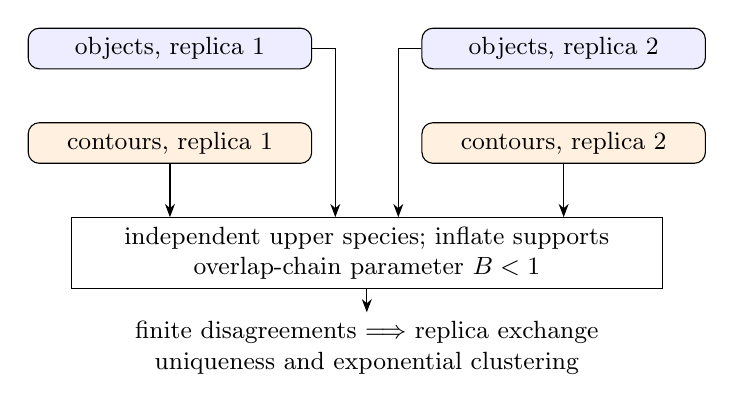
\begin{tikzpicture}[font=\small,>=Stealth]
 \node[draw,rounded corners,fill=blue!7,minimum width=3.6cm] (r1) at (0,1.2) {objects, replica 1};
 \node[draw,rounded corners,fill=orange!12,minimum width=3.6cm] (c1) at (0,0) {contours, replica 1};
 \node[draw,rounded corners,fill=blue!7,minimum width=3.6cm] (r2) at (5,1.2) {objects, replica 2};
 \node[draw,rounded corners,fill=orange!12,minimum width=3.6cm] (c2) at (5,0) {contours, replica 2};
 \node[draw,align=center,minimum width=7.5cm] (b) at (2.5,-1.4) {independent upper species; inflate supports\\overlap-chain parameter $B<1$};
 \coordinate (ml) at (2.1,1.2);\coordinate (mr) at (2.9,1.2);
 \draw[->] (r1.east)--(ml)--(ml |- b.north);
 \draw[->] (r2.west)--(mr)--(mr |- b.north);
 \draw[->] (c1.south)--(c1.south |- b.north);
 \draw[->] (c2.south)--(c2.south |- b.north);
 \node[align=center] at (2.5,-2.6) {finite disagreements $\Longrightarrow$ replica exchange\\uniqueness and exponential clustering};
 \draw[->] (b)--(2.5,-2.15);
\end{tikzpicture}
\caption{The four families are independent because each upper marginal is fixed before mixing over the spins and the reference coupling. Geometric supports may overlap and contour hulls may be nested.}
\label{fig:fourfamilies}
\end{figure}

A disagreement path must run through these covered exceptions. After adding a one-step collar, neighbouring exceptions belong to intersecting supports. A long disagreement therefore requires a long chain in the upper intersection graph. Small occupation probability at a typical site would not suffice: a rare very large support could connect many sites at once. The quantitative parameter below accounts for support size, overlap and diameter. Its bound below one makes every relevant chain component finite, with an exponential tail for its reach.

Now take the union $K$ of disagreement components meeting a fixed local query. When $K$ is finite, exchange the \emph{entire} spin-and-tile labels of the two replicas on $K$. Along its exterior boundary the replicas agree. If $W$ is any crossing-edge weight, $a,b$ the two interior labels and $\tau$ their common exterior label, then
\[
 \underbrace{W(a,\tau)W(b,\tau)}_{\text{before exchange}}
 =\underbrace{W(b,\tau)W(a,\tau)}_{\text{after exchange}}.
\]
Internal factors simply exchange between replicas as well. The product of local weights is unchanged, including hard colour constraints, so the common DLR specification makes the finite exchange probability preserving. It reverses the difference of the two query observables. That difference must have expectation zero, identifying the candidate laws. For two separated queries in one law, the same cancellation fails only when a disagreement component joins them; the exponentially small connection probability then gives clustering. \Cref{lem:swap} supplies the precise finite, random-region argument.

Thus the order of the proof is essential: a certificate selects the reference phase; independent coverings make disagreements finite; only then is the Gibbs exchange legitimate. Finite-box boundary convergence is a separate conclusion, proved in \cref{sec:convergence}.

\subsection{A uniform bias from one witnessed history}
In this subsection $\beta$ is fixed; the bias $h_*$ may depend on $\beta$ and on the witnessed object. Let
\[
 \zeta=\sup_x\sum_{\gamma:\,x\in S_\gamma}w_\gamma<\infty.
\]
The rooted count gives $\zeta\leq16u/(1-16u)$, which may replace $\zeta$ in the lower estimates below. Deleting additional species preserves the following elementary lower bound. For a finite $S$, sequentially require absence of all objects meeting $S$:
\begin{equation}\label{eq:vacancy}
 Q_s(\text{no object meets }S)
 \geq\prod_{\eta:\,S_\eta\cap S\ne\varnothing}(1+w_\eta)^{-1}
 \geq e^{-|S|\zeta}.
\end{equation}
This uses the upper bound on conditional occupation, not stochastic monotonicity of the gas.

Fix spins other than $s_x$. In a finite gas, delete all species marked at $x$ to form a baseline partition function $Z_0$. These deleted species are mutually incompatible, since all contain $x$. Let
\[
 A=\sum_{\gamma:\,x\in M_\gamma}w_\gamma
 r^{N_-(M_\gamma\setminus\{x\},s)}
 Q_0(\text{no object meets }S_\gamma).
\]
Then the two partition functions are $Z_+=Z_0(1+A)$ and $Z_-=Z_0(1+rA)$. These formulas pass to the canonical ratios. If a marked species $\gamma_*$ exists, let $n_*=|S_{\gamma_*}|$ and $k_*=|M_{\gamma_*}|$. Translate one chosen mark to $x$. In the soft case, and in the hard case with its single mark, respectively,
\begin{equation}\label{eq:hstar}
 A\geq A_*:=w_{\gamma_*}r^{k_*-1}e^{-n_*\zeta}>0,
 \qquad h_*:=\frac12\log\frac{1+A_*}{1+rA_*}>0,
\end{equation}
where $r^0=1$ in the hard case. Translation makes this lower bound uniform over $x$. Consequently the spin single-site log odds are bounded below by
\begin{equation}\label{eq:odds-lower}
 \log\frac{\nu(s_x=+\mid s_{x^c})}{\nu(s_x=-\mid s_{x^c})}
 \geq K\sum_{y\sim x}s_y+2(H_x+h_*).
\end{equation}
No quantitative lower bound on $h_*$ independent of the computation is asserted. For an isolated one-mark object of weight $w$, with no competing objects, the spin partition ratio is simply $(1+w)/(1+rw)$, giving a field asymptotic to $(1-r)w/2$ as $w\downarrow0$. The proof uses its strict positivity, not its magnitude.

\subsection{Comparison without target FKG}\label{sec:comparison}
Suppose $\inf_xH_x>-h_*$ and choose $0<\delta\leq\inf_x(H_x+h_*)$. The right side of \eqref{eq:odds-lower} is the log odds of a ferromagnetic Ising reference with uniform field $\delta$. Condition the target on any exterior spins in a finite box, and compare to the reference with minus boundary. Couple single-site heat baths using the same uniforms. If the target configuration is above the reference, its update probability is at least the reference probability evaluated at the target, hence at least that evaluated at the lower reference. This preserves order. Finite positive heat baths converge to their unique stationary kernels. Passing to increasing boxes gives domination of the unique positive-field Ising law.

The reference's uniqueness at $\delta>0$ is the Lebowitz--Martin-L\"of/Lee--Yang consequence specified in \cref{app:imports}. Decreasing the reference field to zero gives the zero-field plus law $\mu_{K,0}^+$. Thus every target spin law in the halting case satisfies
\begin{equation}\label{eq:domplus}
 \nu\succeq\mu_{K,0}^+.
\end{equation}
Only the reference is attractive. Target FKG is unnecessary and does not follow from positive object weights alone. For example, two incompatible objects marked separately at sites $1,2$ give the factor $1+w y_1+w y_2$, with $y_i=1$ for plus and $r$ for minus. Its two-site lattice determinant equals $-w^2(1-r)^2<0$.

Uniformity of the field margin matters. Pointwise positive fields need not suffice: if $H_x>0$ and $\sum_xH_x<\infty$, the bounded positive densities $\exp(\sum_xH_xs_x)$ tilt the two zero-field Ising phases into distinct Gibbs states for that inhomogeneous field. Their distinct tail events persist under equivalent bounded tilts.

\subsection{The reference contour covering}
In a finite plus box, extend all spins by plus. Disagreement bonds form finite even dual-edge graphs. Retain their connected components as graphs, including four-valent vertices, rather than resolving them into loops. Different components are vertex disjoint, and a component of $n$ edges has weight $e^{-Kn}$. The correspondence with plus-exterior spins is exact; deletion of any one component remains admissible, including in nested configurations. Its conditional occupation is therefore at most $e^{-Kn}/(1+e^{-Kn})$, and sequential uniforms dominate the component gas by independent Bernoulli species of parameters $e^{-Kn}$.

Every minus site belongs to the filled hull of some occupied component. A hull of an $n$-edge component has at most $(n+1)^2$ sites and diameter at most $n$. The number of such hull species covering a fixed site is at most
\begin{equation}\label{eq:contourcount}
 (2n+3)^2 16^n,\qquad n\geq4.
\end{equation}
To see this, choose a dual root within distance $n$ and encode the connected edge set by a deterministic doubled-edge traversal of length $2n$. Filled hulls of different components may overlap; independence is asserted for the upper species, not for their geometric hulls. Uniform rooted contour tails permit passage to the infinite plus law: first truncate the contour size around a fixed query, pass to a coupled subsequential limit, then remove the truncation. This proves a coupling of $\mu_{K,0}^+$ to a fixed product contour covering without assuming an infinite-volume contour expansion.

\subsection{Why there really are four independent families}\label{sec:independence}
For each canonical target law couple $s\geq\eta$ with $\eta\sim\mu_{K,0}^+$. Conditional on $s$, sample the objects together with their product upper family $R$ using a kernel depending on $s$ alone. Its $R$ marginal is a fixed product law, independent of $s$. It follows that $R$ is independent of the entire pair $(s,\eta)$: for bounded $F$ and an event $E$,
\[
 \E[F(s,\eta)\one_{R\in E}]=\Prob(R\in E)\E F(s,\eta).
\]
Now draw the upper contour family $C$ conditionally on $\eta$, using fresh randomness from the reference coupling. This preserves independence of $R$ and $C$. Since $s\geq\eta$, the minus sites of $s$ are covered by $C$. The objects are covered by $R$. Repeat the entire construction independently for two independent canonical target states. The resulting families $R_1,C_1,R_2,C_2$ are mutually independent. Merely knowing conditional stochastic domination would not prove this independence.

Inflate each object support and each filled hull by one nearest-neighbour collar. Put a vertex in a graph for every occupied upper species, with edges for intersecting inflated supports. If two canonical replicas disagree at a site, that site is minus in at least one replica or occupied by an object in at least one replica. Every nearest-neighbour disagreement path is therefore covered by an \emph{intersection chain} of inflated supports. This does not identify the intersection graph with the nearest-neighbour components of the union of supports.

For all four families define
\begin{equation}\label{eq:Btotal}
 B=\sup_x\sum_{\xi:\,x\in S_\xi^+}|S_\xi^+|z_\xi2^{\diam S_\xi^+},
\end{equation}
where $z_\xi$ is the upper occupation parameter. The elementary count gives
\begin{align}
 B&\leq200\sum_{n\geq1}n(32u)^n
 +200\sum_{n\geq4}(n+1)^2(2n+3)^2(32e^{-K})^n\nonumber\\
 &<\frac23\qquad(K\geq8,\ u<10^{-4}).\label{eq:Bbound}
\end{align}
The numerical derivation is in \cref{app:estimates}. It applies to the soft table for all $\beta\geq2/5$ and to the hard single-anchor table at $\beta=1$.

A chain reaching distance $R$ from $A$ has total support diameter at least $R$. Apply independence to distinct coloured species, sum over overlap sites, then enlarge to all numerical chains. We obtain
\begin{equation}\label{eq:onearm}
 \Prob(A\text{ has a covering arm to distance }R)
 \leq |A|\frac B{1-B}2^{-R}<2|A|2^{-R},
\end{equation}
and, in particular,
\begin{equation}\label{eq:connection}
 \Prob(A\leftrightarrow B\text{ in disagreements})
 \leq 2|A||B|2^{-\dist(A,B)}.
\end{equation}
The size tails and the arm bound make every relevant occupied intersection component finite, both spatially and in number of species. Hence all site-disagreement components are finite.



\subsection{The finite exchange principle}
We state explicitly the established mechanism being used.
\begin{lemma}[Independent-disagreement exchange]\label{lem:swap}
Let two laws on a finite alphabet satisfy the same nearest-neighbour DLR specification, possibly with hard constraints. If their independent product has only finite nearest-neighbour disagreement components, the laws are equal. For two copies of one such law, and local $f,g$ on $A,B$,
\[
 |\Cov(f,g)|\leq2\norm f_\infty\norm g_\infty
 \Prob(A\leftrightarrow B\text{ in disagreements}).
\]
\end{lemma}
\begin{proof}
Swap replicas on the union $D_A$ of disagreement components meeting $A$. It is finite. Exterior labels on its boundary agree in the replicas. Internal factors exchange, and the product of crossing-edge factors is unchanged, including when a factor is zero. The disagreement set and the choice of $D_A$ are invariant under the swap.

For each deterministic finite set $D$, the product DLR conditional on its exterior is invariant under swapping on the event $D_A=D$. The event is determined by its interior disagreements and agreeing boundary, and is invariant under the same operation. Partition over the countably many finite $D$ to justify the random finite swap. It reverses $f_1-f_2$, proving equality of expectations for any local $f$.

For covariance, use
\[
 \Cov(f,g)=\tfrac12\E[(f_1-f_2)(g_1-g_2)].
\]
On the invariant event that no disagreement component joins $A$ to $B$, the swap reverses the integrand. Its expectation there is zero. On the complement its magnitude is at most $4\norm f_\infty\norm g_\infty$, giving the bound.
\end{proof}

This is the cluster-exchange argument of \cite{VanDenBerg1993}, here proved for the canonical constrained representation. The proof also gives a reusable criterion: any locally decoded finite-object representation with a uniform lower Ising comparison and independent upper object and contour families satisfying \eqref{eq:Btotal} with $B<1$ has at most one canonical spatial Gibbs law, and covariance bounded by $2B/(1-B)$ times the corresponding exponential chain bound. Rectangular computation histories are one way to verify these hypotheses; the exchange itself is not specific to computation.

By \cref{lem:spatialDLR}, all canonical lifts of arbitrary physical Gibbs states satisfy the same specification. Equations \eqref{eq:onearm}--\eqref{eq:connection} and \cref{lem:swap} make these lifts equal. Projection and the unique physical lift then prove full physical uniqueness, not merely translation-invariant uniqueness. They also prove \eqref{eq:maincov}, and the same estimate for local spin-and-tile observables.

\subsection{Transfer to every physical observable}\label{sec:physicalcluster}
Let $F,G$ be bounded physical observables on finite sets $A,B$. Conditional on the complete spins,
\begin{equation}\label{eq:covdecomp}
 \Cov_\mu(F,G)=\E_\nu\Cov(F,G\mid s)
 +\Cov_\nu(\overline F(s),\overline G(s)),\qquad
 \overline F=\E(F\mid s).
\end{equation}
The $b$ variables have independent local conditionals; summing them enlarges the group support by a fixed collar. The first term is exponentially small by \eqref{eq:alpha}. The same influence-path estimate shows that replacing all spins outside $A^\ell$ by plus changes $\overline F$ by at most
\begin{equation}\label{eq:quasilocalF}
 C_A\norm F_\infty\frac{\alpha^{\ell-2}}{1-\alpha},
\end{equation}
with an effectively bounded $C_A$, and analogously for $G$. The truncated conditional means are bounded spin functions. Apply \eqref{eq:maincov} to them, with $\ell=\lfloor\dist(A,B)/4\rfloor$. Their supports grow polynomially in $\ell$ while their separation is at least half the original distance. Absorbing that polynomial gives
\begin{equation}\label{eq:physicalcov}
 |\Cov_\mu(F,G)|\leq C_{A,B}\norm F_\infty\norm G_\infty e^{-c\dist(A,B)},
 \qquad c=\tfrac14\log2,
\end{equation}
with computable support-dependent constants, uniform over inputs and the stated temperatures. Small distances are absorbed by increasing $C_{A,B}$. This proves clustering for the entire physical alphabet, not only for its spin coordinate.

\subsection{The full nonhalting simplex and undecidability}\label{sec:simplex}
Without halting, \eqref{eq:gas} is spin independent. All ratios in \eqref{eq:ratios} are one, so projection and lift identify exactly all zero-field Ising Gibbs laws. At $K\geq8$ the reference is below its critical temperature. An elementary Peierls bound already gives coexistence at $K=7$: using \eqref{eq:contourcount}, its minority bound is less than $121/3072<1/2$. Hence $J_c\leq7/2< K/2$; the exact critical value is unnecessary here.

Coquille--Velenik's Aizenman--Higuchi corollary now applies to this exact two-dimensional nearest-neighbour zero-field Ising specification. Every Ising Gibbs state is $\theta\mu_{K,0}^++(1-\theta)\mu_{K,0}^-$, $0\leq\theta\leq1$. The affine physical lift preserves decompositions and extremality. Its translation covariance proves that every physical Gibbs state is translation invariant. There are exactly two extremal physical states $\mu_M^\pm$.

The plus endpoint has the four-family covering by taking the spin reference itself; the minus endpoint follows by spin reversal of the Ising marginal and the same auxiliary transfer. Thus both cluster for every physical observable. Put $m_K=\mu_{K,0}^+(s_0)$. The contour estimate gives $m_K>0.99$ (indeed the minority probability is less than $10^{-6}$). In an interior mixture,
\begin{equation}\label{eq:mixturecov}
 \Cov(s_0,s_x)=\Cov_{\mu_{K,0}^+}(s_0,s_x)+4\theta(1-\theta)m_K^2.
\end{equation}
The second term is nonzero and the first decays. For the equal mixture, ferromagnetic association makes the covariance at every separation at least $m_K^2>0.99$. At $K=20$ the hard construction has the stronger minority bound recorded in \cref{app:estimates}.

Halting is equivalent to a singleton physical simplex by the preceding proof. Therefore a uniqueness decision algorithm for the exact tables would decide halting. On the machine-indexed promised family the uniqueness predicate is $\Sigma^0_1$-complete and coexistence is $\Pi^0_1$-complete. These are classifications of this effective family, not upper classifications for every finite-range interaction.


% Section: convergence
\section{Finite-volume convergence and its effective scope}\label{sec:convergence}

\subsection{A uniformly computable selected phase}
For a box $V$, define a spin-and-object law $\rho_V^+$ with all exterior spins plus, vacuum exterior tiles, and objects contained in $V$. Its spin weight is the Ising plus-boundary weight times $\Xi_V(s)$. The latter is coordinatewise nondecreasing in the spins, whether or not a marked object exists. The common-uniform heat-bath argument therefore compares the finite spin law from below to the Ising law with the \emph{same plus boundary}. No positive $h_*$ is needed. This remains true for nonnegative inhomogeneous fields.

The two finite contour coverings and two object coverings have the bounds of \cref{sec:selection} uniformly in the volume. Take independent laws in nested boxes $V\subset W$, extending their spin-and-tile configurations by plus and vacuum. They obey the same local specification inside $V$. Exchange disagreement components meeting $A\subset V$ whenever they do not reach $V^c$. Product DLR makes the exchange valid, as in \cref{lem:swap}. Failure requires a covering arm to $V^c$. Thus, for local $f$ on $A$,
\begin{equation}\label{eq:selectedrate}
 |\rho_V^+(f)-\rho_W^+(f)|
 \leq2\norm f_\infty |A|\frac B{1-B}2^{-\dist(A,V^c)}
 <4\norm f_\infty |A|2^{-\dist(A,V^c)}.
\end{equation}
It follows that $\rho_V^+$ converges exponentially to a selected canonical law $\rho^+$. The same comparison for displaced boxes gives translation invariance at uniform field. The replica covariance argument gives clustering. In the nonhalting case its spin law is precisely the Ising plus phase; in the halting case it is the unique spin law.

There is a physical version of this sequence. Include the site factors centred in $V$, sum their $b$ variables and \emph{all} group variables on edges incident to $V$, and impose plus spins outside $V$ for the Ising bonds. By \eqref{eq:gas} its spin marginal is exactly that of $\rho_V^+$. Deep in $V$ its conditional group kernel converges uniformly to $Q_s^g$. The decomposition into conditional means in \cref{sec:physicalcluster}, now using \eqref{eq:selectedrate} and truncation at one quarter of the boundary distance, gives an exponential rate for every fixed local physical observable. All constants can be bounded effectively from its support using \eqref{eq:alpha}. Each limiting local physical DLR identity is valid, so the limit is the physical lift $\mu_M^+$.

For computable $\beta$, the model table and any finite physical expectation are computable by finite enumeration. Given an observable and error, the preceding uniform rate chooses a sufficient box. Thus $\mu_M^+$ is computable uniformly in the machine input, including nonhalting inputs. The required enumeration is enormous and no efficient sampling algorithm is asserted. The free incident group variables are part of the boundary convention; \eqref{eq:selectedrate} is not an estimate for every fixed microscopic boundary.

\subsection{Arbitrary spin boundaries on the halting branch}\label{sec:arbspin}
A stronger, but still qualified, statement is available. Let $\gamma_*$ be a witnessed marked history and choose $d_*$ larger than its diameter plus a fixed collar. In any free-group box $V$, the translated witness lies inside $V$ whenever $x$ is at distance greater than $d_*$ from $V^c$. The finite-volume vacancy argument then gives the same $h_*$ at every such $x$, for arbitrary exterior spins. Set $U=\{x\in V:\dist(x,V^c)>d_*\}$. Conditioning on the spins in $V\setminus U$, the spin law on $U$ dominates the Ising reference with field $h_*$ and minus $U$ boundary.

The following exact reference input is used: Ott \cite[Theorem~6.1, arXiv version~2]{Ott2020} bounds the centre plus/minus magnetization difference in a box of radius $N$, at fixed ferromagnetic coupling and uniform positive field, by $C_0e^{-\nu_0N}$. Our reference coupling is $K/2$ and field $h_*>0$. Domain monotonicity and an inner box centred at $x$ imply an ordered coupling of its finite-minus law $\eta_U^-$ and its infinite positive-field law $\eta_h$ with
\begin{equation}\label{eq:ottmismatch}
 \Prob(\eta_U^-(x)\ne\eta_h(x))
 \leq C_0e^{-\nu_0\dist(x,U^c)}.
\end{equation}
Absorb the factor $1/2$ converting magnetization to mismatch into $C_0$. Glue this to the target domination and to $\eta_h\geq\eta_0^+$. Off the mismatch set, a target minus site is covered by a contour of $\eta_0^+$. The object upper marginal remains independent of the entire reference chain by the constant-marginal construction in \cref{sec:independence}.

For two boxes with arbitrary spin boundaries, let $D=\dist(A,V^c)$ in their common inner box and put $q=D-d_*>0$, $R=\lfloor q/2\rfloor$. For any $x\in A$, a disagreement arm to the boundary either has a four-family covering arm of length $R$, or encounters a reference mismatch in the radius-$R$ buffer about $x$. A union bound over this buffer, not over the whole boundary, gives
\begin{equation}\label{eq:arbbound}
 \Prob(A\text{ has a disagreement arm to }V^c)
 \leq |A|\left[\frac B{1-B}2^{-R}
 +2C_0(2R+1)^2e^{-\nu_0(q-R)}\right].
\end{equation}
For the initial arm, all its covered sites preceding the first mismatch form a chain; thus a mismatch encountered after that chain leaves the buffer is already counted by the first term. Finite exchange inside the common box now proves exponential convergence uniformly over spin boundaries. Transfer to physical observables uses conditional group mixing exactly as before.

The constants in this conclusion depend on the witnessed history, $K$, and the positive-field reference constants. We have not extracted numerical $C_0,\nu_0$. This proves existence of a model-dependent exponential rate for \emph{free incident group variables and arbitrary spin boundaries}. It is not arbitrary microscopic-boundary mixing or strong spatial mixing.

\subsection{A general effective compactness theorem}\label{sec:modulus}
There is a useful general limitation on what ``noncomputable convergence despite uniqueness'' can mean.

\begin{theorem}[A valid modulus under the uniqueness promise]\label{thm:effectivemodulus}
Let a finite-alphabet finite-range finite-energy specification on $\Z^d$ have computable local kernels, with its finite alphabet and a finite-range bound supplied effectively. If it has a unique Gibbs state, that state and a valid local all-boundary convergence modulus are computable. One uniform partial algorithm terminates on every such unique input. The assertion includes computable translation-invariant finite tables at computable temperature.
\end{theorem}
\begin{proof}
Fix a finite observable support $A$ and nested boxes $V_n\supset A$. Finite range means that the marginal kernel on $A$ depends on the exterior only through a finite boundary collar. Define the computable real
\[
 D_n(A)=\max_{\tau,\tau'}\TV\bigl((\gamma_{V_n}^\tau)_A,(\gamma_{V_n}^{\tau'})_A\bigr).
\]
The maximum is over finitely many collar assignments and consists of finite positive sums. If $D_n(A)$ does not tend to zero, choose boundary pairs separated by a fixed amount along a subsequence. Compactness gives two subsequential limiting laws. Every fixed DLR identity passes to these limits by locality; they are Gibbs states with different $A$ marginals, contradicting uniqueness.

Search over $n$ and rational precision for a strict certificate $D_n(A)<\varepsilon$. Approximation to the finitely many probabilities semidecides this strict inequality. Under uniqueness the search terminates. Its certificate is valid for every larger box and every Gibbs law: by conditioning on the collar of $V_n$, any such $A$ marginal is a convex mixture of the inner kernels whose diameter was bounded. The same is true for every larger-volume boundary assignment. Hence any one inner kernel approximates the unique marginal, and the certificate controls convergence for all larger boxes, not just the first one found.

Dovetail this construction over finite supports and errors $2^{-k}$. It computes both the state and a valid modulus. No proof of uniqueness is required as input; termination uses the uniqueness promise.
\end{proof}

For general computable finite-range specifications, this also gives a $\Pi^0_2$ upper description of uniqueness: for each finite support in an exhaustion and each $k$, there is a finite strict-diameter certificate below $2^{-k}$. The strict numerical certificate has a decidable finite witness. No completeness claim for this general upper bound is made.

\begin{proposition}[No total family-wide minus-boundary bound]\label{prop:nototal}
There is no total computable function of the machine input returning a box size beyond which the free-group, minus-spin finite-volume mean is within $1/4$ of its infinite-volume value on every halting input. The function is not required to be valid on nonhalting inputs. The same impossibility holds for an all-boundary bound.
\end{proposition}
\begin{proof}
On every nonhalting input, the finite spin law is exactly minus-boundary zero-field Ising and has centre mean less than $-0.99$ at every box size, by reference monotonicity. On every halting input the unique infinite-volume mean exceeds $0.99$, by \eqref{eq:domplus}. If the total function existed, evaluate the finite mean at its output size to error $1/8$. The result is negative on every nonhalting input and positive on every halting input. This decides halting, a contradiction. For a bound stated for actual physical DLR boxes, enlarge the returned box by a fixed collar of width two. The natural law then contains every interaction meeting the inner box; conditioning on its physical collar gives the exact inner DLR kernel. Its query marginal is a mixture of those kernels and obeys the all-boundary certificate. The same finite computation again decides halting.
\end{proof}

Thus a fixed unique computable model does not furnish a noncomputable valid convergence modulus. The obstruction is to a total rule across this undecidable family. The plus sequence \eqref{eq:selectedrate} is a positive exception precisely because it selects an equilibrium on both branches.


% Section: pressure
\section{Pressure, smooth response and one-sided computability}\label{sec:pressure}

For a uniform dimensionless field $h$, define the physical pressure using counting measure on the full alphabet:
\[
 p_\beta(h)=\lim_{L\to\infty}\frac1{L^2}\log Z_{[1,L]^2}^{\rm free}(h),
\]
where the free Hamiltonian includes terms wholly contained in the box. Finite range gives existence and independence of ordinary boundary conventions. Normalized Haar integration used earlier changes only explicit spin-independent normalising constants, never the derivatives in $h$.

\subsection{Pressure values and slopes}
For our nonnegative physical terms, tiling large boxes by $L$-boxes and deleting crossing terms gives
\begin{equation}\label{eq:pressurecompute}
 p_L(h)-\frac{42\beta}{L}\leq p_\beta(h)\leq p_L(h),\qquad
 p_L(h)=L^{-2}\log Z_{[1,L]^2}^{\rm free}(h).
\end{equation}
Indeed at most $2L$ site factors and $2L$ mismatch bonds per block cross the tiling; their energies are at most $1$ and $20$. Remainders vanish in the thermodynamic limit. The field terms are on-site and create no crossing error. Finite positive partition sums are computable, so \eqref{eq:pressurecompute} computes the pressure uniformly for computable $\beta,h$. This elementary estimate is a special case of established pressure computability results; it is not an undecidability of the pressure value.

The finite-alphabet full-shift variational principle identifies translation-invariant Gibbs laws with equilibrium laws for finite-range interactions; precise hypotheses are checked in \cref{app:imports}. Consequently
\begin{equation}\label{eq:slopes}
 p_\beta'(h-)=\min_{\mu\in\Gibbs_{\rm TI}(h)}\mu(s_0),\qquad
 p_\beta'(h+)=\max_{\mu\in\Gibbs_{\rm TI}(h)}\mu(s_0).
\end{equation}
For completeness, pressure is the supremum of the affine functions
$\mathsf h(\mu)-\beta e(\mu)+h\mu(s_0)$ on the compact invariant measure space. Entropy is upper semicontinuous on a finite full shift and energy is continuous. Taking maximisers at $h+t$ along $t\downarrow0$ gives a maximiser at $h$; comparing the two variational inequalities identifies the right derivative as the maximum slope of these maximisers. The left derivative is the minimum, by the same argument.

On the nonhalting branch, \eqref{eq:gas} implies
\[
 p_\beta(h)=c_\beta+p^{\rm Ising}_K(h)
\]
with a spin-independent $c_\beta$. In the soft case this includes the nontrivial unmarked-gas pressure. Hence $p_\beta'(0\pm)=\pm m_K$. On the halting branch the unique state has positive magnetization exceeding $0.99$, so both slopes coincide and are positive. Thus differentiability at zero is equivalent to halting.

\subsection{Fixed-order cumulants from local clustering}
For bounded random variables $X_1,\ldots,X_n$, write
\[
 \kappa_n(X_1,\ldots,X_n)=
 \sum_{\pi\in\mathcal P_n}(|\pi|-1)!(-1)^{|\pi|-1}
 \prod_{C\in\pi}\E\prod_{i\in C}X_i,
\]
where $\mathcal P_n$ is the set of partitions of $\{1,\ldots,n\}$.

\begin{lemma}[Summable cumulants]\label{lem:cumulant}
Any class of spin laws satisfying \eqref{eq:maincov} uniformly obeys, for $n\geq2$,
\begin{equation}\label{eq:cumulantbound}
 |\kappa_n(s_{x_1},\ldots,s_{x_n})|
 \leq C_n2^{-\diam\{x_1,\ldots,x_n\}/(n-1)},\qquad
 C_n=4n^2\sum_{\pi\in\mathcal P_n}|\pi|!.
\end{equation}
Every fixed-order cumulant is absolutely summable over relative positions, with a computable uniform tail.
\end{lemma}
\begin{proof}
For positive diameter, remove a longest edge from a minimum spanning tree on the indexed positions. Its length $a$ is at least the diameter divided by $n-1$. The resulting parts $I,J$ have every cross-distance at least $a$, since a shorter crossing edge would improve the tree. Replace the joint law by the product of its $I$ and $J$ marginals. Its mixed cumulant is zero.

In the moment formula, a block meeting both parts changes by a covariance of two spin products, of magnitude at most $4n^2 2^{-a}$ by \eqref{eq:maincov}; noncrossing blocks do not change. Every moment has magnitude at most one. Telescoping products for a partition with $|\pi|$ blocks, then multiplying by $(|\pi|-1)!$, yields \eqref{eq:cumulantbound}. Repeated positions cannot lie across a positive-distance cut. At diameter zero the elementary moment bound is smaller than $C_n$.

With $x_1=0$, tuples whose maximum radius is $m$ number at most $(2m+1)^{2(n-1)}$. An explicit tail beyond radius $R$ is therefore
\begin{equation}\label{eq:cumulanttail}
 C_n\sum_{m\geq R}(2m+1)^{2(n-1)}2^{-m/(n-1)}.
\end{equation}
For each fixed $n$ this converges geometrically after a computable initial segment, uniformly over the class.
\end{proof}

\subsection{The inhomogeneous-field bridge to response}\label{sec:response}
Infinite-volume clustering alone does not justify differentiating a thermodynamic limit. Here the missing uniformity follows from the proof: on a halting input, uniqueness and \eqref{eq:maincov} hold for \emph{every bounded field profile} with infimum greater than $-h_*$. This includes arbitrary finite field tilts, with the same covariance and cumulant constants.

\begin{proposition}[Smooth pressure]\label{prop:smooth}
On a halting input, for either stated construction and temperature,
$p_\beta\in C^\infty((-h_*,\infty))$. For $n\geq2$,
\begin{equation}\label{eq:derivatives}
 p_\beta'(h)=\mu_h(s_0),\qquad
 p_\beta^{(n)}(h)=\sum_{x_2,\ldots,x_n\in\Z^2}
 \kappa_{n,h}(s_0,s_{x_2},\ldots,s_{x_n}).
\end{equation}
The sums converge absolutely and locally uniformly. In particular $0\leq p_\beta''(h)\leq68$.
\end{proposition}
\begin{proof}
For finite $\Lambda$ let $\mu_{\Lambda,t}$ be the probability law with density proportional to $\exp(t\sum_{x\in\Lambda}s_x)$ relative to $\mu_h$. The local DLR equations identify it as a Gibbs law with field $h+t\one_\Lambda$. Uniqueness identifies it with the unique law for that profile. Finite differentiation gives, for local $F$,
\begin{equation}\label{eq:finiteresponse}
 \frac d{dt}\mu_{\Lambda,t}(F)
 =\sum_{x\in\Lambda}\Cov_{\mu_{\Lambda,t}}(F,s_x).
\end{equation}
On a compact $t$-interval inside the permitted range, local subsequential limits as $\Lambda\uparrow\Z^2$ satisfy the uniform-field DLR equations and equal $\mu_{h+t}$. Convergence is uniform in $t$: otherwise take a convergent sequence of parameters witnessing failure and apply the same compactness argument. Uniform clustering bounds the sum tails in \eqref{eq:finiteresponse}. Passing to the integrated identity proves differentiability of local moments and its infinite response sum.

For higher orders, finite-tilt differentiation of a cumulant adds one spin variable summed over $\Lambda$. Apply \cref{lem:cumulant} at each fixed order. Uniform local moment convergence and \eqref{eq:cumulanttail} justify passage through the integrated identity, including the sums in all relative positions. Induction with the fundamental theorem of calculus proves every derivative in \eqref{eq:derivatives}; it does not formally differentiate an uncontrolled infinite series. The first identity follows from \eqref{eq:slopes} and uniqueness. Finally convexity gives $p''\geq0$, and
\[
 p''(h)\leq4\sum_{x\in\Z^2}2^{-\norm x_\infty}
 =4\left(1+8\sum_{m\geq1}m2^{-m}\right)=68.
\]
\end{proof}

This is a concrete use of the classical cumulant-response mechanism, rather than a new general implication from clustering. The available $C_n$ do not imply an $n!C^n$ derivative bound. We assert no analyticity or convergent Taylor series for the target model.

\subsection{The computable right jet and the noncomputable left slope}
For every input, including nonhalting ones, all bounded field profiles with positive infimum give uniqueness: use \eqref{eq:odds-lower} with $h_*=0$ if no certificate is available. The clustering estimates are uniform as the positive uniform field decreases to zero. The selected finite-volume estimate \eqref{eq:selectedrate} is also uniform for $h\geq0$. Since finite-volume probabilities are continuous in $h$, their uniform limit $\mu_h^+$ is locally right-continuous at zero. Uniform cumulant tails give the same continuity for each sum in \eqref{eq:derivatives}.

Apply the finite-tilt response argument on $h>0$ and pass through its integrated identities to the endpoint. Every right derivative of pressure at zero exists, and equals the cumulant sum of the selected zero-field plus state (with $n=1$ interpreted as magnetization). This is a smooth one-sided jet; it need not determine pressure on any neighbourhood.

The jet is uniformly computable. For order $n\geq2$, choose a radius using \eqref{eq:cumulanttail}; enumerate the finitely many remaining tuples and partitions; compute their selected local moments with \eqref{eq:selectedrate} to sufficient total accuracy. The cases $n=1$ and $n=0$ use the selected mean and \eqref{eq:pressurecompute}. All choices terminate without deciding halting.

In contrast, \eqref{eq:slopes} gives
\[
 p_\beta'(0-)=\begin{cases}
  -m_K<-0.99,&\text{without halting},\\
  \mu_M(s_0)>0.99,&\text{with halting}.
 \end{cases}
\]
A uniform computation of this real number even to error $1/4$ would decide halting by its sign. This is a family-wise noncomputability statement, compatible with computability of each pressure value, the selected phase, its complete right jet, and the valid modulus under a uniqueness promise.


% Section: stability
\section{Perturbations and exact restoration of coexistence}\label{sec:stability}

\subsection{Spin-only multibody perturbations}
Add to the exponent a finite-range interaction $\sum_X\Psi_X(s_X)$; translation invariance and ferromagnetism are not required. Put
\[
 d_X=\osc(\Psi_X),\qquad
 \delta=\sup_x\sum_{X\ni x}d_X,\qquad
 p_X=1-e^{-d_X},
\]
and, with $X^+$ the nearest-neighbour collar, define the two-replica activation parameter
\begin{equation}\label{eq:Bpsi}
 B_\Psi=2\sup_x\sum_{X:\,x\in X^+}|X^+|p_X2^{\diam X^+}.
\end{equation}
Use $B_0$ for the unperturbed bound in \eqref{eq:Bbound}.

\begin{theorem}[A spin perturbation neighbourhood]\label{thm:spinpert}
On a halting input, at a uniform field $h$, suppose
\begin{equation}\label{eq:pertconditions}
 h+h_*>\delta/2,\qquad B_0+B_\Psi<1.
\end{equation}
Then the perturbed physical model has exactly one Gibbs state, exponentially clustering for every bounded local physical observable. For spin observables its covariance is bounded by
\[
 \frac{2B}{1-B}\norm f_\infty\norm g_\infty|A||C|2^{-\dist(A,C)},
 \qquad B=B_0+B_\Psi.
\]
If $\diam X\leq R$, a sufficient condition is
\begin{equation}\label{eq:explicitradius}
 \delta<\min\{h+h_*,(6C_R)^{-1}\},\quad
 C_R=10v_R2^{R+2},\quad v_R=\min\{5(R+1)^2,(R+3)^2\}.
\end{equation}
These are perturbations of the distinguished spins only.
\end{theorem}
\begin{proof}
A one-site log odds changes by at most $\sum_{X\ni x}d_X\leq\delta$. Thus the lower reference field is $h+h_*-\delta/2>0$. Comparison with the zero-field plus reference still holds, without any sign assumption on $\Psi$.

For each finite support, write the positive expansion
\begin{equation}\label{eq:activation}
 e^{\Psi_X(s_X)}=e^{\min\Psi_X}\,[1+q_X(s_X)],\qquad
 q_X=e^{\Psi_X-\min\Psi_X}-1\geq0.
\end{equation}
Conditional on the spins, introduce independent activation variables with probability $q_X/(1+q_X)\leq p_X$. Multiplying the spin weight by their conditional kernels cancels the factors $1+q_X$: the augmented weight has factor $q_X(s_X)$ when active and $1$ when inactive, apart from a spin-independent constant. This cancellation remains valid where $q_X=0$; no strictly positive likelihood ratio between activation laws is presumed.

Use fresh uniforms for a product activation upper family whose law, conditional on the complete spins and all previous variables, is fixed with parameters $p_X$. It is therefore independent of the four families in \cref{sec:independence}. Two replicas add two independent families. Their inflated intersection parameter is \eqref{eq:Bpsi}, so the same chain estimate holds with $B=B_0+B_\Psi<1$.

For exchange, include the entire support of every occupied object and every active factor in the actual bad hypercomponents, together with minus sites in both replicas, joining neighbouring sites and incident supports. Entire active supports must be used even if disconnected. Each such component lies in a finite component of the six upper families. Swap spins, whole objects and activation labels on the finite union of components meeting the query. No object or active factor crosses its boundary. Every inactive crossing factor contributes $1$, and an internal active factor exchanges its full spin pattern and activation label. Thus augmented product weights, including zeros, are preserved. One may verify the same identity by finite removal, spin change and reinsertion, as in \cref{lem:spatialDLR}; this avoids dividing by a zero activation weight. Partition over the finite regions and finite object/factor lists to justify the random exchange. The covariance and uniqueness proof of \cref{lem:swap} now applies verbatim to these hypercomponents. Physical group conditionals remain unchanged, so \cref{sec:physicalcluster} transfers clustering.

Finally $|X^+|\leq v_R$, $\diam X^+\leq R+2$, and $x\in X^+$ implies $X$ meets the five-site nearest-neighbour neighbourhood of $x$. Since $p_X\leq d_X$, this gives $B_\Psi\leq C_R\delta$. Under \eqref{eq:explicitradius}, $B<2/3+1/6=5/6$ and the field margin remains positive.
\end{proof}

In physical energy units $\Psi=-\beta W$. For each fixed range and each witnessed halting input this gives an explicit open spin neighbourhood. It does not control perturbations of the multiplicity or group tables.

\subsection{Arbitrarily small microscopic symmetrization}\label{sec:symmetry}
The preceding scope cannot simply be replaced by a uniform radius for arbitrary physical perturbations.

\begin{proposition}[No family-wide real-potential radius]\label{prop:symmetrize}
At $\beta=1$, for every $\varepsilon>0$ there is a halting input whose unperturbed physical interaction, in either construction, admits a translation-invariant real-valued perturbation on the same supports of norm below $\varepsilon$ with at least two Gibbs states. Here the norm is $\sup_x\sum_{X\ni x}\norm{W_X}_\infty$.
\end{proposition}
\begin{proof}
For one site let $U=\sum_{z\text{ unmarked}}\mathcal X_z$ and $V=\sum_{z\text{ marked}}\mathcal X_z$, with $m$ marked tile types. The two summed factors are
\[
 f_+=1+a_\beta p(U+V),\qquad
 f_-=1+a_\beta(pU+qV).
\]
At $\beta=1$, put $f_{\rm sym}=(f_++f_-)/2$ and add the $b$-independent physical site energy
\begin{equation}\label{eq:symenergy}
 \Delta(s,g)=\log\frac{f_s(g)}{f_{\rm sym}(g)}.
\end{equation}
Its multiplicity sum is exactly $C_\beta f_{\rm sym}$, independent of $s$. The group factor stays in $[1-u,1+u]$ and has the same Dobrushin estimate. The summed system is therefore the product of a unique group law and zero-field Ising. Lift either Ising phase and restore the local multiplicity kernels to obtain distinct physical Gibbs states. Moreover,
\begin{equation}\label{eq:symnorm}
 \norm\Delta_\infty\leq\frac{a_\beta(p-q)m}{2(1-u)}.
\end{equation}
Each site lies in at most three translated site-factor supports; the interaction norm is at most three times this quantity.

It remains to make $m/t$ small while keeping halting. Start with a one-step-halting machine whose initial state is not halting, and add unreachable states. Let $P$ be the number of ordered tape-symbol pairs and $Q$ the number of machine states. For either permanent-bit value the folded cell alphabet has
\[
 \sigma_0=P(1+2Q)+1,\qquad \sigma=2\sigma_0
\]
letters, including poison. Interior-row, interior-column tiles alone give $t\geq\sigma^2\sigma_0$: their neighbour letters are arbitrary, their centre has bit zero, and their visible edge data distinguish the choices. For the hard grammar the marked types number $m=3P\sigma$, whence
\[
 \frac mt\leq\frac{3}{8PQ^2}\longrightarrow0.
\]
For the soft grammar, bottom rows have no halting centre for this chosen initial word. In the other two row types, the possible halting centres and column statuses give the safe bound
\[
 m\leq4P\sigma^2+8P\sigma,\qquad
 \frac mt\leq\frac{8P}{\sigma}+\frac{16P}{\sigma^2}\longrightarrow0.
\]
These counts follow directly from the explicit tuples in \cref{app:compiler}; in particular they survive deduplication of identical visible tile data. Padding changes no reachable transition and thus no genuine history. Since $a_\beta<1/[10000(pt+1)]$, \eqref{eq:symnorm} tends effectively to zero. Choose enough unreachable states to make the interaction norm less than $\varepsilon$.
\end{proof}

The perturbations are finite computable \emph{real} tables. A constant shift can make them nonnegative without changing Gibbs laws, at the cost of at most a factor two in the norm bound. This result does not concern a topology restricted to integer-valued tables, and it does not exclude a physical perturbation neighbourhood for each fixed halting input. Nor does it establish a first-order transition under a small uniform negative field: selection of plus at one field and minus at another would not by itself prove coexistence between them.


% Section: discussion
\section{Scope and further questions}\label{sec:discussion}

The construction separates three questions that can otherwise look similar. A selected clustered phase is uniformly computable. Uniqueness among all Gibbs states is undecidable. Under a uniqueness promise, a valid all-boundary convergence modulus is computable by a partial search. The obstruction is therefore not a failure to compute each individual unique equilibrium. It is the inability to recognise uniformly that no competing equilibrium exists, or to supply certain total convergence guarantees across both branches.

The physical model uses one distinguished Ising spin and a large finite auxiliary alphabet. It is not a two-state spin model. With dimension, finite supports, alphabet and a finite allowed set of energy values all fixed, there are only finitely many tables, so an unbounded halting reduction needs an input channel. Here the alphabet supplies that channel. Reducing its size, replacing the threshold multiplicity encoding by a smaller positive representation, or obtaining nearest-neighbour pair interactions without an implicit hard constraint remains open.

The dimension also has a clear role. A translation-invariant one-dimensional finite-table finite-energy interaction has a primitive transfer representation after finite blocking and hence a unique Gibbs state. Such a class cannot provide the coexistence branch used here. Uniform boundedness or translation invariance matters in this observation; merely requiring each term of a spatially unbounded inhomogeneous one-dimensional interaction to be finite is insufficient.

The soft construction simplifies the computational grammar and eliminates proof pins, but retains exact character cancellation. A genuinely different exact-integer finite-temperature reduction remains desirable. Merely giving a finite program for a computable real coupling changes the representation: a small positive Ising field can then encode halting through its name, but an algorithm outputting its exact numerator and denominator would already decide the zero-versus-positive question. Such an encoding does not replace the finite-table theorem.

Several probabilistic extensions are unresolved. We do not prove analyticity of the target pressure, exponential convergence for arbitrary fixed microscopic auxiliary boundaries, strong spatial mixing, a spectral gap for Glauber dynamics, or robustness to all sufficiently small physical perturbations of a fixed model. The finite-object exchange controls equilibrium disagreements, not time-dependent relaxation. The reference Ising theorems giving analyticity or stronger mixing cannot simply be transferred to a target lacking their ferromagnetic structure. To settle these questions one would need, respectively, controlled growth of cumulant constants, a treatment of fixed auxiliary boundary layers, a dynamical coupling, or a quantitative norm bound on induced spin interactions under microscopic perturbation.

The central finite-certificate mechanism is more general than its implementation: exact positive realisation produces a canonical finite-object representation; one witnessed object supplies a uniform bias; an ordered reference controls one kind of defect; an independent sparse covering controls the remaining objects; finite exchange removes all competing canonical Gibbs states. The construction verifies this chain for exact finite-temperature tables and all physical Gibbs states. The constituent Ising, comparison, exchange and thermodynamic principles retain their established provenance.


% Section: acknowledgements
\section*{Acknowledgements and AI use}
\label{sec:acknowledgements}
The mathematical ideas, constructions, proofs, and manuscript were developed by GPT-6 Astra, with additional AI assistance for review. Human input was minimal and consisted primarily of setting the research objectives and providing occasional feedback.

\appendix

% Section: compiler
\section{An explicit compiler for finite computation rectangles}
\label{appcomp:section}
\label{app:compiler}

This appendix gives two effective finite Wang-tile compilers.  The first
produces only accepting finite components and marks their top-left corners.
The second permits every finite initial history and marks every occurrence
of a halting head.  The machine simulation and rectangle geometry are the
same in both cases.  These are statements about \emph{finite components};
no exclusion of infinite matching configurations is asserted.

\begin{proposition}[Finite-component compiler]
\label{appcomp:compiler}
Given a deterministic Turing machine and a finite input, one can compute a
finite set of labelled Wang tiles, a finite edge-colour alphabet with a
distinguished colour $0$, and a set of marked tile types, with the following
properties.  Adjoin a vacuum letter having colour $0$ on all four edges.
In any matching configuration on $\mathbb Z^2$, connect two nonvacuum
tiles when their common edge has nonzero colour.  Every finite connected
component is a solid rectangle of width and height at least two, whose rows
are successive states of the prescribed initial computation on a finite
tape interval, with an absorbing rejection on overflow.
\begin{enumerate}
\item In the \emph{accepting version}, the top row contains a halting head,
and the component has precisely one marked tile, its top-left corner.
A finite component exists if and only if the given machine halts.
\item In the \emph{history version}, no terminal acceptance condition is
imposed.  A tile is marked precisely when its centre letter carries a
halting head.  A finite \emph{marked} component exists if and only if the
given machine halts.  Unmarked components are allowed.
\end{enumerate}
The output is obtained by enumerating finite sets and evaluating finite
transition tables.  In particular the compiler does not test whether a
halting computation or a marked rectangle exists.
\end{proposition}

\subsection{A folded, bounded-width deterministic simulation}
\label{appcomp:folding}

Let $\Gamma$ be the finite tape alphabet, with blank symbol $\square$.
Normalize the machine so that it starts in state $q_0$ at tape position
$0$, the input is written at positions $0,1,\ldots$, and all other positions
are blank.  Its tape is indexed by $\mathbb Z$.  Replace all genuine halting
outcomes by one absorbing state $\mathrm{HALT}$.  Complete the transition
table on all other state--symbol pairs, using $\mathrm{HALT}$ for a missing
transition if that is the original machine's halting convention.  Add a
\emph{new} absorbing state $\mathrm{REJECT}$, reserved for finite-interval
overflow.  Thus an original halting outcome is never confused with the
overflow state.  Allow moves in $\{-1,0,+1\}$; an unused stay-put move causes
no change to the construction.

Fold the two-sided tape onto positions $j\geq0$.  Position $j$ stores a pair
$(A_j,B_j)\in\Gamma^2$, representing original positions $j$ and $-j-1$,
respectively.  A head has a state and a track $\tau\in\{A,B\}$.  Each cell
also has an immutable origin bit $o$, which is $1$ at $j=0$ and $0$
elsewhere.  An original transition writes only the currently selected
component of the pair.  Its physical motion and new track are as follows:
\begin{center}
\begin{tabular}{c|c|c|c}
track & original move & physical move & new track\\ \hline
$A$ & $+1$ & $+1$ & $A$\\
$A$ & $-1$, $o=0$ & $-1$ & $A$\\
$A$ & $-1$, $o=1$ & $0$ & $B$\\
$B$ & $-1$ & $+1$ & $B$\\
$B$ & $+1$, $o=0$ & $-1$ & $B$\\
$B$ & $+1$, $o=1$ & $0$ & $A$\\
$A$ or $B$ & $0$ & $0$ & unchanged
\end{tabular}
\end{center}
The new machine state is the state prescribed by the original transition.
For $\mathrm{HALT}$ and $\mathrm{REJECT}$, the update preserves the head,
track and tape symbols.  One original step is one folded step, including
a track change at the origin.

On an interval $\{0,\ldots,W-1\}$, a proposed physical move through a wall
is instead replaced by a $\mathrm{REJECT}$ head at its source, after the
prescribed write.  Overflow takes precedence even if the original
transition proposed the new state $\mathrm{HALT}$.  This may reject a narrow
certificate, but never accepts an invalid one.  Every finite genuine
computation fits a sufficiently wide interval.

The finite cell alphabet is
\begin{equation}
\label{appcomp:cellalphabet}
\Sigma=
\bigl(\Gamma^2\times\{0,1\}\times
 (\{\text{no head}\}\cup(Q\times\{A,B\}))\bigr)
 \ \cup\ \{\bot_0,\bot_1\},
\end{equation}
where $Q$ includes the two absorbing states.  The poison letter $\bot_o$
retains origin bit $o$.  Let $\#$ be a wall symbol not in $\Sigma$.

\subsection{A completely specified radius-one update}
\label{appcomp:localupdate}

Define a deterministic finite map
\begin{equation}
\label{appcomp:Fdomain}
F:(\Sigma\cup\{\#\})\times\Sigma\times
       (\Sigma\cup\{\#\})\longrightarrow\Sigma .
\end{equation}
Only triples whose centre lies in $\Sigma$ are used.  For a nonpoison head
letter, its own state, selected tape symbol, track and origin bit determine
its prescribed write, proposed new state and track, and physical
displacement.  These data are computable from that letter alone.

For a triple $(p,x,q)$, apply the following rules in the displayed order.
\begin{enumerate}
\item If any nonwall entry is poison, output the poison letter with the
centre's origin bit.
\item Form the centre's new tape pair: perform its prescribed write if it
has a head, and otherwise retain its old pair.  Copy its origin bit.
\item An \emph{incoming proposal} comes from $p$ if $p$ has a head whose
physical displacement is $+1$, and from $q$ if $q$ has a head whose
physical displacement is $-1$.  Each proposal carries that head's
prescribed new state and track.  If there are two incoming proposals,
or if an incoming proposal meets a centre that already carries a head,
output poison with the centre's origin bit.
\item If there is exactly one incoming proposal, install its state and
track on the centre's new tape pair.
\item Otherwise, if the centre has no head, retain a headless centre.  If
it has a head with displacement zero, retain its prescribed new head.
If it moves toward an actual neighbouring cell, leave its source
headless.  If it moves toward a wall $\#$, retain an absorbing
$\mathrm{REJECT}$ head at the source.  Use the source track in this last
case.
\end{enumerate}
These alternatives define every triple in \eqref{appcomp:Fdomain}.
For configurations reached from the specified one-head initial row,
the poison cases never occur.  A direct check shows that a head either
stays, transfers to one neighbouring cell, changes track at the origin,
or becomes the single absorbing overflow head.  Therefore there remains
exactly one head and the parallel update is precisely the folded
finite-interval simulation.  Soundness below uses this invariant, rather
than any intended interpretation of malformed histories.

\subsection{The row automata}
\label{appcomp:automata}

Let $P=P_0\cdots P_{\ell-1}$ be the folded input prefix, where
$\ell\geq1$ is large enough to include the entire input and the head at
cell zero.  At cell zero the origin bit is one and the initial head is
$(q_0,A)$; all other prefix cells are headless and have origin bit zero.
Unused tape components are blank.  Write $z$ for the blank, headless,
origin-bit-zero letter.  The initial-row language is exactly
\begin{equation}
\label{appcomp:bottomlanguage}
Pz^* .
\end{equation}
Its deterministic finite automaton has states
$0,1,\ldots,\ell$ and a rejecting sink.  At $i<\ell$, the only
nonrejecting transition reads $P_i$ and goes to $i+1$.  At $\ell$, the
only nonrejecting transition reads $z$ and stays at $\ell$.  The start
state is $0$ and the sole accepting state is $\ell$.  All other
transitions go to the sink.  In particular a proper prefix of $P$ is
not accepted.

For the accepting version, the top-row automaton has states
$u,a,d$, meaning unseen, seen and dead.  A headless nonpoison letter
leaves $u$ or $a$ unchanged.  A $\mathrm{HALT}$ head changes $u$ to $a$,
and changes $a$ to $d$.  Every other head and every poison letter goes
to $d$; $d$ remains $d$ on every letter.  The start state is $u$ and
the sole accepting state is $a$.  Its language consists of words with
exactly one halting head and otherwise ordinary headless letters.

For the history version, the top automaton has one accepting state
with a loop on every letter of $\Sigma$.  In both versions the
interior-row automaton is this one-state automaton.  The geometry
below requires the origin bit of each centre letter to be one exactly
in the leftmost column, independently of the row automata.

\subsection{The complete finite tile generator}
\label{appcomp:tiles}

Use horizontal statuses $\eta\in\{L,I,R\}$ and vertical statuses
$\nu\in\{B,I,T\}$.  The letters $L,R$ are distinct, as are $B,T$.
A candidate tile is a tuple
\begin{equation}
\label{appcomp:tuple}
(\eta,\nu,p,x,q,k_-,k_+),
\end{equation}
where $x\in\Sigma$, $p,q\in\Sigma\cup\{\#\}$, and $k_-,k_+$
are states of the automaton assigned to row status $\nu$.
Enumerate all such tuples and retain exactly those satisfying:
\begin{enumerate}
\item $p=\#$ if and only if $\eta=L$, and $q=\#$ if and only if
$\eta=R$;
\item the origin bit of $x$ is one if and only if $\eta=L$;
\item $k_+$ is the automaton transition from $k_-$ on $x$, and neither
state is rejecting or dead;
\item if $\eta=L$, then $k_-$ is the start state;
\item if $\eta=R$, then $k_+$ is an accepting state.
\end{enumerate}
Put $y=F(p,x,q)$.  Give the retained tile the colours
\begin{align}
\label{appcomp:colours}
 c_W&=\begin{cases}0,&\eta=L,\\
 (\mathrm{hor},\nu,p,x,k_-),&\eta\ne L,
 \end{cases}
&c_E&=\begin{cases}0,&\eta=R,\\
 (\mathrm{hor},\nu,x,q,k_+),&\eta\ne R,
 \end{cases}\\
 c_S&=\begin{cases}0,&\nu=B,\\
 (\mathrm{ver},\eta,x),&\nu\ne B,
 \end{cases}
&c_N&=\begin{cases}0,&\nu=T,\\
 (\mathrm{ver},\eta,y),&\nu\ne T.
 \end{cases}\nonumber
\end{align}
The two tags $\mathrm{hor}$ and $\mathrm{ver}$ are distinct formal
symbols.  Every displayed tuple is a nonzero colour.  The colour $0$
is different from every tuple, including tuples containing a blank,
a wall symbol or the numerical automaton state $0$.

In the accepting version mark a tile exactly when $(\eta,\nu)=(L,T)$.
In the history version mark it exactly when $x$ has a
$\mathrm{HALT}$ head.  The tile set consists of these retained labelled
tuples.  Distinct retained tuples can be kept as distinct labelled types
even if their four colours happen to coincide.  All subsequent tile
counts and activities must count those labels consistently.  No
deduplication or minimization is needed for the theorem.

\subsection{Geometry, soundness and completeness}
\label{appcomp:proof}

\begin{proof}[Proof of Proposition~\ref{appcomp:compiler}]
Take a finite nonzero-edge component and a tile at its lowest vertical
coordinate.  Its south edge must be zero, hence its vertical status is
$B$.  Following nonzero horizontal edges cannot continue indefinitely.
It therefore yields an entire row starting with $L$, ending with $R$,
and having only $I$ statuses between them.  Matching horizontal colours
force one common vertical status and a matching automaton run along
the row.  A gap or a premature endpoint would put a zero colour against
a nonzero colour.  Because $L$ and $R$ are distinct, the row has width
at least two.

Every tile of this bottom row has a nonzero north edge.  Vertical
matching produces the row above, carrying the same horizontal statuses
and therefore exactly the same horizontal extent.  Its common vertical
status is $I$ or $T$, since its south edges are nonzero.  Repeat this
argument.  Finiteness forces a top row of status $T$.  The distinction
between $B$ and $T$ gives height at least two.  The resulting rectangle
has colour zero on its entire exterior boundary, so no further tile
can connect to it.  In particular no hole, branch, ragged row or extra
piece of the component is possible.  Other components can touch it
only across zero-coloured edges.

Let $x_0\cdots x_{W-1}$ be the centre letters in a row.  Horizontal
matching in \eqref{appcomp:colours} gives
$p_i=x_{i-1}$ and $q_i=x_{i+1}$ at the internal positions, with
$p_0=q_{W-1}=\#$ at the two walls.  The automaton states match as well.
The bottom row is therefore exactly \eqref{appcomp:bottomlanguage}.
Vertical matching forces each next centre letter to be
$F(x_{i-1},x_i,x_{i+1})$, with wall symbols at the ends.  The origin-bit
condition is correct at every height.  The initial one-head invariant
from Section~\ref{appcomp:localupdate} now identifies every row with
the genuine bounded-width computation.  Poison cannot appear.

In the accepting version the top automaton requires a halting head.
An overflow head remains $\mathrm{REJECT}$ forever, so acceptance
certifies a genuine halt before any wall failure.  Exactly one tile
has statuses $(L,T)$, giving the unique marked anchor.  In the history
version a mark is itself a genuine halting head in one of these rows.
There is no requirement that such a head be unique among the rows:
the absorbing halt may occur in several successive rows.  Unmarked
finite histories, including histories that eventually overflow, are
permitted.  Thus the indicated accepting or marked component always
implies genuine halting.

Conversely suppose the original computation halts after finitely many
steps.  Choose $W\geq\max(2,\ell)$ large enough to contain all folded
positions used up to and including that transition.  The finite-interval
simulation then reaches $\mathrm{HALT}$ without overflow.  Stack its
initial row and all successive images through a halting row, repeating
the absorbing halt if needed to make the height at least two.  Assign
statuses $B$ to the first row, $T$ to the last, $I$ between them, and
$L,I,R$ to the columns.  The stored triples and the row automata give
exactly the retained tiles above.  They match vertically and
horizontally, and their exterior colours are zero.  This is a finite
accepting component in the first version and a finite marked history
component in the second.  Every step of the construction is finite
and effective, completing the proof.
\end{proof}

\begin{remark}[The distinction between the two versions]
\label{appcomp:distinction}
On a nonhalting input the accepting version has no finite nonvacuum
component.  The history version generally has many finite components,
but none is marked.  Consequently its positive object partition
function is spin independent in the nonhalting case, rather than
necessarily equal to one.  The accepting version supports a hard
single-anchor spin eligibility.  The history version uses a positive
marked-site penalty in the main construction, which allows multiple
marks without allowing a minus spin at a different mark to forbid the
entire witness.  This appendix changes neither the stated physical
integer energies nor the finite-energy requirement: tile matching is
used only in the proof representation.
\end{remark}

\begin{remark}[Infinite sectors are not excluded]
\label{appcomp:infinite}
The all-interior blank tile is a simple example of a tile that can
match itself on the whole plane.  Such an infinite component is
compatible with the grammar even on a halting input.  The proposition
therefore does not assert uniqueness of the hard-tile specification
under arbitrary tile boundaries.  In the physical model, arbitrary
Gibbs states are related to the canonical finite-object law by a
separate positive auxiliary-variable mixing argument; the finite
compiler alone does not justify that passage.
\end{remark}


% Section: estimates
\section{Counting and quantitative covering estimates}\label{app:estimates}

\subsection{Rooted counts and collars}
A connected $n$-site support containing $x$ has a deterministic spanning tree. A fixed rooted traversal of that tree is a nearest-neighbour walk of length $2(n-1)$ and determines its visited support. There are at most $4^{2(n-1)}\leq16^n$ such walks. Multiplication by $t^n$ bounds labelled objects. Their diameter is at most $n$, so
\[
 \sup_x\sum_{\gamma:\,x\in S_\gamma}|S_\gamma|w_\gamma2^{\diam S_\gamma}
 \leq\sum_{n\geq1}n(32u)^n.
\]
For a connected $n$-edge dual graph, a deterministic traversal of its doubled edges gives at most $16^n$ graphs through a specified dual vertex. If its filled hull contains a fixed primal site, one can choose a dual vertex in a square of at most $(2n+3)^2$ possible locations. The hull has diameter at most $n$ and cardinality at most $(n+1)^2$. These intentionally loose bounds include four-valent crossings and nested hulls.

For either object supports or hulls, one-step inflation costs at most five in rooted count, five in cardinality, and four in the weight $2^{\diam}$. Two replicas therefore cost at most $2\cdot5\cdot5\cdot4=200$. This proves the two series in \eqref{eq:Bbound}. The first factor five comes from choosing a site in the nearest-neighbour neighbourhood of the query lying in the uninflated support; it is distinct from the cardinality factor five.

\subsection{Exact numerical bounds}
Put $a=32/10000=2/625$. Then
\[
 2\sum_{n\geq1}na^n=\frac{2500}{388129}<0.006442,
 \qquad 200\sum_{n\geq1}na^n=\frac{250000}{388129}.
\]
The partial exponential series gives $e>163/60>19/7$, and $(19/7)^8>2560$. Thus, for $K\geq8$, $32e^{-K}<1/80$. If $P_n=(n+1)^2(2n+3)^2$, then for $n\geq4$,
\[
 \frac{P_{n+1}}{P_n}\leq(6/5)^2(13/11)^2<9/4,\qquad P_4=3025.
\]
Consequently
\[
 200\sum_{n\geq4}P_n(32e^{-K})^n
 <\frac{200\cdot3025\cdot80^{-4}}{1-9/320}
 =\frac{605}{39808},
\]
and
\begin{equation}\label{eq:exactB}
 B< b_0:=\frac{250000}{388129}+\frac{605}{39808}
 =\frac{10186818045}{15450639232}<\frac23.
\end{equation}
These bounds use no temperature-dependent choice of the physical table. They prove the entire finite half-line $\beta\geq2/5$ for the soft table. There is no assertion at $\beta=\infty$, where positivity is lost, or that $2/5$ is optimal.

The minority probability in the Ising plus phase does not require the hull-cardinality factor. By the contour covering,
\[
 \delta_I\leq\sum_{n\geq4}(2n+3)^2(16e^{-K})^n.
\]
The polynomial ratio is below $2$ for $n\geq4$. At $K\geq8$,
\begin{equation}\label{eq:minority}
 \delta_I<\frac{121\cdot160^{-4}}{1-2/160}
 =\frac{121}{647168000}<10^{-6}.
\end{equation}
At $K=7$, the weaker $e>2$ gives $\delta_I<121/3072<1/2$, establishing coexistence below the reference values used in the main theorems. At the hard table's $K=20$, $16e^{-20}<2^{-16}$ gives
\[
 \delta_I<\frac{121\cdot2^{-64}}{1-2^{-15}}<10^{-16}.
\]
In particular the hard table's equal-mixture spin covariance is at least $1-4\delta_I>0.99$ at every separation, even without association: a union bound in the plus phase gives $\E s_0s_x\geq1-4\delta_I$, and spin reversal leaves that two-point function unchanged.

\subsection{Weighted chains and one-arm bounds}
For clarity, let independent Bernoulli species have parameters $z_\xi$ and finite supports $T_\xi$, and suppose
\[
 b=\sup_x\sum_{\xi:\,x\in T_\xi}|T_\xi|z_\xi2^{\diam T_\xi}<1.
\]
For a distinct-species intersection chain from $x$ to $y$, the sum of support diameters is at least $\dist(x,y)$. Independence bounds its probability by the product of parameters. To sum chains, choose an initial support containing $x$; choose an exit site in it; choose the next support containing that site; and continue. After multiplying by $2^{\sum\diam}$, every step is bounded by $b$. A final factor $|T_\xi|\geq1$ can be inserted harmlessly. Thus chains of length $k$ contribute at most $b^k2^{-\dist(x,y)}$.

For an arm to distance $R$, the same argument stops at its first reach of that distance. It yields $\sum_{k\geq1}b^k2^{-R}$ directly, without summing over all possible endpoints. Independence was applied only to distinct species; the geometric numerical sum is enlarged by allowing repetitions. Local finiteness follows from $\sum_{\xi:x\in T_\xi}z_\xi<\infty$. The one-arm estimate excludes infinite spatial components; local finiteness then excludes infinitely many species in a finite component. These statements justify both the finite gas exchange and the finite replica swaps.


% Section: imports
\section{Exact interfaces with established theorems}\label{app:imports}

This appendix records the mathematical hypotheses of the imported results and where they hold. The direct arguments in the text are retained so that no unproved transfer from the reference Ising model to the target is implicit.

\subsection{Conditional Dobrushin comparison}
Rebeschini--van Handel \cite[Corollary~2.6, arXiv version~1]{RebeschiniVanHandel2014} gives the classical single-site comparison bound. With influence matrix $C$, local update discrepancies $b_j$, and $D=\sum_{n\geq0}C^n$, the difference of expectations is bounded by $\sum_{i,j}\osc_i(f)D_{ij}b_j$, subject to quasilocal reference kernels and the stated vanishing-$C^n$ condition. Finite discrete single-site spaces satisfy its metric and topological hypotheses. This is a modern precise formulation of the classical Dobrushin theorem \cite{Dobrushin1968}.

Here the index set is the countable edge set of $\Z^2$, each site space is a finite group, the single-edge heat-bath kernels are local and positive, and \eqref{eq:alpha} gives $\norm C_\infty\leq\alpha<1$. Thus row sums of $C^n$ are at most $\alpha^n$ and the vanishing condition holds. Equal specifications have $b=0$, giving uniqueness. Remote boundary or spin modifications create discrepancies only where the local factors change, so the resolvent sum starts at the corresponding path distance. Conditioning on a finite set, or local positive tilting followed by approximation, gives the conditional covariance consequences used in \eqref{eq:covdecomp}. Multiplicity restoration is a local independent kernel. None of this compares the low-temperature spins by Dobrushin's criterion.

\subsection{Positive-field Ising and zero-field classification}
Lebowitz--Martin-L\"of \cite[Theorem~1]{LebowitzMartinLof1972} treats translation-invariant summable nonnegative Ising pair interactions with a uniform field (and allows a periodic background). It identifies uniqueness with differentiability in the uniform field. Its explicit consequence on p.~278, from Lee--Yang \cite{LeeYang1952}, is uniqueness at nonzero homogeneous field when the background is zero. Their boundary comparison, in particular Lemma~2, sandwiches arbitrary finite-boundary correlations between plus and minus limits. It supplies the all-DLR formulation: condition any DLR law on a box and let the equal plus/minus limits exhaust it.

Our reference has nearest-neighbour $J=K/2>0$, absolutely summable nonnegative pair couplings, zero background and uniform $\delta>0$. Every hypothesis therefore holds. Reference monotonicity and the limit as $\delta\downarrow0$ identify the plus law used in \eqref{eq:domplus}. Holley's finite-lattice criterion \cite{Holley1974} is a standard comparison route, but we do not leave a target/reference lattice inequality unchecked: the ordered heat-bath proof in \cref{sec:comparison} proves precisely the needed comparison without target FKG.

Coquille--Velenik \cite[Corollary~1.1]{CoquilleVelenik2012} states that for the nearest-neighbour zero-field ferromagnetic Ising model on $\Z^2$ at $J>J_c$, the set of \emph{all} DLR measures is exactly the segment between the plus and minus states. No translation-invariance hypothesis on the input state is required. Our nonhalting projection is that exact specification, and \cref{app:estimates} verifies $J\geq4>J_c$. The affine inverse lift in \cref{sec:allprojection} transfers the entire segment, extremality and translation invariance. This classification is an application of Aizenman--Higuchi, not a new general Ising theorem.

\subsection{Independent disagreement and the object gas}
Van den Berg \cite[Theorem~1, p.~162]{VanDenBerg1993} assumes a countable connected locally finite graph, finite or countable site spaces, and two Markov fields with the same specification. If their independent product has no infinite disagreement path, the laws coincide. Its proof on p.~163 exchanges finite disagreement clusters. Our graph is $\Z^2$, the spin-and-tile site space is finite, and \cref{lem:spatialDLR} verifies the common nearest-neighbour specification for all canonical physical lifts. The independent covering estimate then verifies absence of infinite disagreements. The direct proof in \cref{lem:swap} is this established exchange, with its covariance consequence. It is applied pairwise within the canonical class, not to unrelated infinite-component tile states.

Van den Berg--Maes \cite[Theorem~1 and Corollaries~1--2]{VanDenBergMaes1994} provide finite-volume disagreement coupling and percolation criteria using worst-conditional one-site discrepancies. Their small-percolation criterion is not automatically met here. At $\beta=1$, vacuum neighbouring tiles and all-plus versus all-minus neighbouring spins already give spin-conditional variation $\tanh(40)$. Our upper families instead describe rare typical defects after a phase comparison.

For an alternative canonical-gas construction, Ferrari--Fern\'andez--Garcia \cite[Theorem~1(ii)]{FerrariFernandezGarcia2002} constructs the stationary birth/death process from finite free-process ancestor clans. Their discrete branching criterion in equations (4.3)--(4.4) is
\[
 \sup_\gamma\frac1{q(\gamma)}\sum_\eta q(\eta)\lambda_\eta I(\gamma,\eta)<1,
 \qquad \inf_\gamma q(\gamma)\geq1.
\]
Take countably many finite labelled objects, self-including overlap incompatibility, death rate one, birth rates $a_\eta(s)\leq w_\eta$, and $q(\gamma)=|S_\gamma|$. The left side is at most
\[
 \sup_x\sum_{\eta:\,x\in S_\eta}|S_\eta|w_\eta
 \leq\sum_{n\geq1}n(16u)^n<0.001606.
\]
Rooted free birth intensities are finite. Common Poisson cylinders therefore construct finite ancestor clans for any finite query. Detailed balance identifies finite restrictions with the product-activity gas. Common ancestor constructions remove finite cutoffs; the diameter-weighted bound $\sum_n n(32u)^n<0.003221$ gives exponential locality by generation paths. These last quantitative estimates are the applicability calculation, not extra statements quoted from that theorem. The incompatibility graph has infinite degree, so a locally finite graph theorem should not be applied directly on its species vertices.

The Section~2 Theorem of Koteck\'y--Preiss \cite{KoteckyPreiss1986} is another optional route. With size function $a(\gamma)=|S_\gamma|$, its incompatibility summability criterion holds even for activities inflated by $e^{|S_\gamma|}$, since
\[
 \sum_{\eta\sim\gamma}w_\eta e^{2|S_\eta|}
 \leq |S_\gamma|\sum_{n\geq1}(16ue^2)^n<|S_\gamma|.
\]
Here $u<10^{-4}$ and $e<3$ suffice; deleting or reducing activities preserves the bound. We use neither the resulting logarithmic expansion nor an induced-potential reconstruction. The static finite exchange is sufficient.

\subsection{Reference boundary estimate}
Ott \cite[Theorem~6.1, arXiv:1905.12928v2]{Ott2020} fixes nearest-neighbour ferromagnetic Ising on $\Z^d$ with exponent coupling nonnegative and uniform $h>0$. It bounds the plus/minus centre magnetization difference in $[-N,N]^d$ by $Ce^{-\nu N}$, where $C<\infty$ and $\nu>0$ depend on the reference parameters. We use $d=2$, coupling $K/2$, field $h_*>0$, strictly within these hypotheses. Inner-box monotonicity gives \eqref{eq:ottmismatch}. The query-buffer and swap proof of \eqref{eq:arbbound} is supplied here; the target is not itself an Ising model. Ott's analyticity theorems are not imported for the target.

\subsection{Variational pressure and smoothness}
Barbieri--G\'omez--Marcus--Taati \cite[Theorem~1.1(a),(b), Proposition~3.2; arXiv version~2]{BarbieriGomezMarcusTaati2020} supplies the Gibbs/equilibrium and pressure interfaces. The Gibbs-to-equilibrium direction assumes a finite-alphabet $\Z^d$ subshift with D-mixing and an absolutely summable interaction; the reverse direction assumes finite type. Proposition~3.2 uses a standard Borel environment, relative topological Markov property and D-mixing along a F\o lner sequence. For us the environment is a singleton, the physical configuration space is the finite full shift, all patterns paste freely, boxes are F\o lner, and the interaction is finite range. Every hypothesis is immediate on this \emph{physical} shift; no such claim is needed for constrained proof tiles. It follows that the free partition-function limit is the invariant variational pressure and that its maximisers are precisely invariant physical Gibbs states. Equation \eqref{eq:slopes} is then proved directly.

Lebowitz \cite[Section~I, (1.12)--(1.13); Section~II, (2.4a,b), pp.~317--318]{Lebowitz1972Correlations} is a predecessor for fixed-order Ursell decay and smoothness from uniformly summable derivatives; this general discussion is unnumbered. Lebowitz--Penrose \cite[Section~VII, (90)--(93)]{LebowitzPenrose1968} supplies a further classical thermodynamic precedent. The target's finite-support inhomogeneous-tilt argument is proved in \cref{sec:response}, rather than assuming ferromagnetic hypotheses it does not have.

Gayral--Sablik--Taati \cite[Proposition~14]{GayralSablikTaati2025} proves computability of pressure for computable potentials on finite-alphabet full shifts; the present table meets those hypotheses. Equation \eqref{eq:pressurecompute} is a direct elementary certificate in this special class. Their Proposition~15 concerns effective invariant equilibrium sets, rather than a chosen microscopic boundary sequence. Fawzi--Fawzi--Scalet \cite[Theorems~2.1--2.4, published numbering]{FawziFawziScalet2024} gives certified equilibrium-observable intervals, invariant refinements, a strict all-states sign promise algorithm, and quantitative commuting high-temperature/one-dimensional bounds. Our diagonal interaction fits the commuting setting, but its nonhalting magnetization signs violate that strict sign promise. Target clustering alone does not meet their high-temperature criterion. No quantitative result from these theorems is used in our finite-volume proof.

\bibliographystyle{amsplain}
\providecommand{\bysame}{\leavevmode\hbox to3em{\hrulefill}\thinspace}
\providecommand{\MR}{\relax\ifhmode\unskip\space\fi MR }
% \MRhref is called by the amsart/book/proc definition of \MR.
\providecommand{\MRhref}[2]{%
  \href{http://www.ams.org/mathscinet-getitem?mr=#1}{#2}
}
\providecommand{\href}[2]{#2}
\begin{thebibliography}{10}

\bibitem{BarbieriGomezMarcusTaati2020}
Sebasti{\'a}n Barbieri, Ricardo G{\'o}mez, Brian Marcus, and Siamak Taati,
  \emph{Equivalence of relative {Gibbs} and relative equilibrium measures for
  actions of countable amenable groups}, Nonlinearity \textbf{33} (2020),
  no.~5, 2409--2454.

\bibitem{Berger1966}
Robert Berger, \emph{The undecidability of the domino problem}, Memoirs of the
  American Mathematical Society, no.~66, American Mathematical Society,
  Providence, RI, 1966.

\bibitem{BinderHeLiZhang2025}
Ilia Binder, Qiandu He, Zhiqiang Li, and Yiwei Zhang, \emph{On computability of
  equilibrium states}, International Mathematics Research Notices \textbf{2025}
  (2025), no.~6, rnaf055.

\bibitem{CoquilleVelenik2012}
Loren Coquille and Yvan Velenik, \emph{A finite-volume version of
  {Aizenman--Higuchi} theorem for the 2d {Ising} model}, Probability Theory and
  Related Fields \textbf{153} (2012), no.~1-2, 25--44.

\bibitem{CubittPerezGarciaWolf2022}
Toby~S. Cubitt, David P{\'e}rez-Garc{\'i}a, and Michael~M. Wolf,
  \emph{Undecidability of the spectral gap}, Forum of Mathematics, Pi
  \textbf{10} (2022), e14.

\bibitem{Dobrushin1968}
R.~L. Dobrushin, \emph{The description of a random field by means of
  conditional probabilities and conditions of its regularity}, Theory of
  Probability and Its Applications \textbf{13} (1968), no.~2, 197--224.

\bibitem{FawziFawziScalet2024}
Hamza Fawzi, Omar Fawzi, and Samuel~O. Scalet, \emph{Certified algorithms for
  equilibrium states of local quantum {Hamiltonians}}, Nature Communications
  \textbf{15} (2024), 7394.

\bibitem{FerrariFernandezGarcia2002}
Pablo~A. Ferrari, Roberto Fern{\'a}ndez, and Nancy~L. Garcia, \emph{Perfect
  simulation for interacting point processes, loss networks and {Ising}
  models}, Stochastic Processes and their Applications \textbf{102} (2002),
  no.~1, 63--88.

\bibitem{GayralSablikTaati2025}
L{\'e}o Gayral, Mathieu Sablik, and Siamak Taati, \emph{Characterisation of the
  set of ground states of uniformly chaotic finite-range lattice models},
  Nonlinearity \textbf{38} (2025), no.~7, 075011.

\bibitem{GuPerales2012}
Mile Gu and {\'A}lvaro Perales, \emph{Encoding universal computation in the
  ground states of {Ising} lattices}, Physical Review E \textbf{86} (2012),
  no.~1, 011116.

\bibitem{GuWeedbrookPeralesNielsen2009}
Mile Gu, Christian Weedbrook, {\'A}lvaro Perales, and Michael~A. Nielsen,
  \emph{More really is different}, Physica D: Nonlinear Phenomena \textbf{238}
  (2009), no.~9-10, 835--839.

\bibitem{HochmanMeyerovitch2010}
Michael Hochman and Tom Meyerovitch, \emph{A characterization of the entropies
  of multidimensional shifts of finite type}, Annals of Mathematics
  \textbf{171} (2010), no.~3, 2011--2038.

\bibitem{Holley1974}
Richard Holley, \emph{Remarks on the {FKG} inequalities}, Communications in
  Mathematical Physics \textbf{36} (1974), no.~3, 227--231.

\bibitem{Kanter1990}
I.~Kanter, \emph{Undecidability principle and the uncertainty principle even
  for classical systems}, Physical Review Letters \textbf{64} (1990), no.~4,
  332--335.

\bibitem{KoteckyPreiss1986}
Roman Koteck{\'y} and David Preiss, \emph{Cluster expansion for abstract
  polymer models}, Communications in Mathematical Physics \textbf{103} (1986),
  no.~3, 491--498.

\bibitem{LebowitzPenrose1968}
J.~L. Lebowitz and O.~Penrose, \emph{Analytic and clustering properties of
  thermodynamic functions and distribution functions for classical lattice and
  continuum systems}, Communications in Mathematical Physics \textbf{11}
  (1968), no.~2, 99--124.

\bibitem{Lebowitz1972Correlations}
Joel~L. Lebowitz, \emph{Bounds on the correlations and analyticity properties
  of ferromagnetic {Ising} spin systems}, Communications in Mathematical
  Physics \textbf{28} (1972), no.~4, 313--321.

\bibitem{LebowitzMartinLof1972}
Joel~L. Lebowitz and Anders Martin-L{\"o}f, \emph{On the uniqueness of the
  equilibrium state for {Ising} spin systems}, Communications in Mathematical
  Physics \textbf{25} (1972), no.~4, 276--282.

\bibitem{LeeYang1952}
T.~D. Lee and C.~N. Yang, \emph{Statistical theory of equations of state and
  phase transitions. {II}. lattice gas and {Ising} model}, Physical Review
  \textbf{87} (1952), no.~3, 410--419.

\bibitem{Ott2020}
S{\'e}bastien Ott, \emph{Weak mixing and analyticity of the pressure in the
  {Ising} model}, Communications in Mathematical Physics \textbf{377} (2020),
  no.~1, 675--696.

\bibitem{RebeschiniVanHandel2014}
Patrick Rebeschini and Ramon van Handel, \emph{Comparison theorems for {Gibbs}
  measures}, Journal of Statistical Physics \textbf{157} (2014), no.~2,
  234--281.

\bibitem{VanDenBerg1993}
J.~van~den Berg, \emph{A uniqueness condition for {Gibbs} measures, with
  application to the 2-dimensional {Ising} antiferromagnet}, Communications in
  Mathematical Physics \textbf{152} (1993), no.~1, 161--166.

\bibitem{VanDenBergMaes1994}
J.~van~den Berg and C.~Maes, \emph{Disagreement percolation in the study of
  {Markov} fields}, The Annals of Probability \textbf{22} (1994), no.~2,
  749--763.

\bibitem{Wolfram1985}
Stephen Wolfram, \emph{Undecidability and intractability in theoretical
  physics}, Physical Review Letters \textbf{54} (1985), no.~8, 735--738.

\end{thebibliography}

\end{document}
